\documentclass[12pt]{report}
\usepackage[italian]{babel}
\usepackage[most]{tcolorbox}
\usepackage{amsmath}
\usepackage{amsthm}
\usepackage{mathtools}
\usepackage{tabularx}
\usepackage{amssymb}
\usepackage{enumitem}
\usepackage{amsfonts}
\usepackage{centernot}
\usepackage{relsize}
\usepackage{mathrsfs}
\usepackage{bm}
\usepackage{xfrac}
\usepackage{lipsum}
\usepackage{bbm}
\usepackage{tikz}
\usepackage{cancel}
\usepackage{enumitem}
\usepackage{mathtools}
\usepackage{multicol}
\usepackage{float}
\usepackage{hyperref}
\usepackage{makecell}
\usepackage{listings}
\usepackage{xcolor}
\usepackage{pgfplots}
\usepackage{calligra}
\usepackage[toc,page]{appendix}
\usepackage{tikz}
\usepackage{yhmath}
\usetikzlibrary{angles, quotes, patterns}
\usepackage{circledsteps}
\date{}
\author{Alessandro Carella}
\title{Calcolo delle probabilita' e statistica}
\setcounter{chapter}{0}
\setlist[enumerate]{label*=\arabic*.}
\setlength{\parindent}{0pt}
\definecolor{brickred}{RGB}{182, 50, 28}
\definecolor{darkred}{RGB}{139, 0, 0}
\hypersetup{
	colorlinks=true,
	linkcolor=darkred,
	filecolor=darkred,
	urlcolor=darkred
}

\newcounter{theorem}
\newcounter{lemma}
\newcounter{corollary}
\newcounter{definition}
\newcounter{exercise}

\labelformat{theorem}{teorema #1}
\labelformat{lemma}{lemma #1}
\labelformat{corollary}{corollario #1}
\labelformat{definition}{definizione #1}
\labelformat{note}{nota #1}
\labelformat{example}{esempio #1}
\labelformat{exercise}{esercizio #1}

\newtcbtheorem[number within=chapter,use counter=theorem]{theorem}%
{Teorema}{arc=1mm,outer arc=1mm,colframe=cyan!55!black,fonttitle=\scshape,lefttitle=1mm,separator sign dash,description font=\bfseries,description delimiters={\flqq}{\frqq}}{th}

\newtcbtheorem[number within=theorem,use counter=corollary]{corollary}%
{Corollario}{arc=1mm,outer arc=1mm,colframe=cyan!55!black,fonttitle=\scshape,lefttitle=1mm,separator sign dash,description font=\bfseries,description delimiters={\flqq}{\frqq}}{cor}

\newtcbtheorem[number within=chapter,use counter=lemma]{lemma}%
{Lemma}{arc=1mm,outer arc=1mm,colframe=cyan!55!black,fonttitle=\scshape,lefttitle=1mm,separator sign dash,description font=\bfseries,description delimiters={\flqq}{\frqq}}{lem}

\newtcbtheorem[number within=chapter,use counter=definition]{definition}%
{Definizione}{breakable, enhanced, arc=1mm,outer arc=1mm,colframe=green!55!black,fonttitle=\scshape,separator sign dash,description font=\bfseries,description delimiters={\flqq}{\frqq}}{def}

\newtcbtheorem[no counter]
{note}{Nota}{blanker,breakable,left=5mm,before skip=10pt,after skip=10pt,borderline west={2.5mm}{0pt}{red!55},coltitle=black,fonttitle=\bfseries}{note}

\newtcbtheorem[no counter]
{example}{Esempio}{blanker,breakable,left=5mm,before skip=10pt,after skip=10pt,borderline west={2.5mm}{0pt}{yellow!55},coltitle=black,fonttitle=\bfseries}{exa}

\newtcbtheorem[number within=section,use counter=exercise]
{exercise}{Esercizio}{blanker,breakable,left=5mm,before skip=10pt,after skip=10pt,borderline west={2.5mm}{0pt}{yellow!55},coltitle=black,fonttitle=\bfseries}{exe}

\newtcbtheorem[no counter]
{assignment}{Traccia}{blanker,breakable,left=5mm,before skip=10pt,after skip=10pt,borderline west={2.5mm}{0pt}{brickred!65},coltitle=black,fonttitle=\bfseries}{asg}
\tcolorboxenvironment{proof}{blanker,breakable,left=5mm,before skip=10pt,after skip=10pt,borderline west={2.5mm}{0pt}{cyan!55!black}}
\newcommand{\namerefl}[1]{%
	\bgroup
	\let\nmu\MakeLowercase
	\nameref{#1}\egroup}

\newcommand{\nmu}{}

\begin{document}
	{
		\let\cleardoublepage\clearpage
		\maketitle
		\tableofcontents
	}
	\chapter{Spazio di probabilita'}
	\begin{definition}{\nmu Spazio di probabilita'}{spazio_prob}
		Lo spazio di probabilita' e' una terna $(\Omega, \mathcal{F}, P)$.
		\begin{enumerate}
			\item $\Omega$ e' un insieme non vuoto, lo spazio campionario, i cui elementi $\omega \in \Omega$ rappresentano i singoli esiti dell'esperimento aleatorio;
			\begin{example}{}{}
				Esperimento di lancio di una moneta: \\
				$\Omega = \{T,\ C\}$ \\
				Lancio di un dado: \\
				$\Omega = \{1, 2, 3, 4, 5, 6\}$
			\end{example}
			\item $\mathcal{F} \subset \mathcal{P}(\Omega) \quad (|\mathcal{P}(\Omega)| = 2^{|\Omega|})$ e' una collezione di sottoinsiemi di $\Omega$, chiamati \textbf{eventi}, tali che:
			\begin{enumerate}
				\item $\emptyset, \Omega \in \mathcal{F}$ ove $\emptyset$ e' l'evento impossibile e $\Omega$ e' l'evento certo;
				\item $E \in \mathcal{F} \iff E^C = \Omega \backslash E \in \mathcal{F}$
				\item Se $\{E_n\}_{n \in \mathbbm{N}} \subset \mathcal{F}$ e' una successione di eventi $\Rightarrow \mathlarger{\bigcup^{\infty}_{n=1}}E_n \in \mathcal{F}$ \\
				Ad esempio: \\
				$E_1, E_2 \in \mathcal{F} \Rightarrow E_1 \cup E_2 \in \mathcal{F}$ \\ \\
				Ne consegue la seguente proprieta':
				\item $E_1, E_2 \in \mathcal{F} \Rightarrow E_1 \cap E_2 \in \mathcal{F}$ \\
				Infatti, dalle legge di De Morgan ne consegue che: \\
				$(E_1 \cap E_2)^C = E_1^C\ \cup E_2^C \in \mathcal{F}$ \\
				Piu' in generale, se $\{E_n\ : n \in \mathbbm{N}\} \subset \mathcal{F} \Rightarrow \mathlarger{\bigcap^\infty_{n=1}}E_n \in \mathcal{F}$
 			\end{enumerate}
 			\textbf{$\mathcal{F}$ e' una $\sigma$-algebra se rispecchia le proprieta' elencate}.
 			\item $P$ e' una funzione di probabilita', cioe':
 			\[
 			P: \mathcal{F} \to [0, 1]
 			\]
 			\[
 			E \mapsto \mathcal{P}(E) \in \mathcal{F}
 			\]
 			tale che:
 			\begin{enumerate}
 				\item $\mathcal{P}(\emptyset) = 0, \mathcal{P}(\Omega) = 1$
 				\item Se $\{E_n\ : n \in \mathbbm{N}\} \subset \mathcal{F}$ con $E_n \cap E_m = \emptyset \quad \forall n \neq m$ \\
 				\[\mathcal{P}\Bigg(\bigcup^\infty_{n=1}E_n\Bigg) = \sum_{n=1}^{\infty}\mathcal{P}(E_n)\]
 				Di conseguenza:
 				\begin{itemize}
 					\item $\mathcal{P}(E^C) = 1 - \mathcal{P}(E)$\\
 					Questo perche': \[\Omega = E\ \cup E^C \Rightarrow \mathcal{P}(\Omega) = \mathcal{P}(E\ \cup E^C) \Rightarrow 1 = \mathcal{P}(E) + \mathcal{P}(E^C)\]
 					\item Sia $E_2 \subset E_1$ \\ $\mathcal{P}(E_1 \backslash E_2) = \mathcal{P}(E_1) - \mathcal{P}(E_2) \geq 0 \iff \mathcal{P}(E_1) \geq \mathcal{P}(E_2)$ \\
 					Questa e' la \textbf{monotonia}: \[E \subseteq F \in \mathcal{F} \Rightarrow \mathcal{P}(E) \leq \mathcal{P}(F)\]
 					\item $\mathcal{P}(E_1 \cup E_2) = \mathcal{P}(E_1) + \mathcal{P}(E_2) - \mathcal{P}(E_1 \cap E_2)$ \\
 					Questo perche':
 					\[
 					E_1 \cup E_2 = E_1 \cup (E_2 \backslash E_1) \Rightarrow \mathcal{P}(E_1 \cup E_2) = \mathcal{P}(E_1) + \mathcal{P}(E_2 \backslash E_1)
 					\]
 					\[
 					E_2 \backslash E_1 = E_2 \backslash (E_1 \cap E_2) \Rightarrow \mathcal{P}(E_2 \backslash E_1) = \mathcal{P}(E_2) - \mathcal{P}(E_1 \cap E_2)
 					\]
 					Ne consegue che:
 					\[
 					\mathcal{P}(E_1 \cup E_2) \leq \mathcal{P}(E_1) + \mathcal{P}(E_2)
 					\]
 				\end{itemize}
 			\end{enumerate}
		\end{enumerate}
	\end{definition}
	\section{Esempi di spazi di probabilita'}
	\subsection{Spazi finiti}
	Negli spazi di probabilita' finiti $\Omega$ e' un insieme finito, ovvero: $|\Omega| < \infty$.
	Una distribuzione di probabilita' finita su $\Omega$ e' una probabilita' $P$ tale che $\mathcal{P}(\{\omega\}) = p$, dove $\omega \in \Omega$ e $p$ e' un numero che non dipende da $\omega$. Dalla relazione:
	\[
	1 = \mathcal{P}(\Omega) = \sum_{w \in \Omega}\mathcal{P}(\{w\}) = \sum_{p = \mathcal{P}(\{w\})}p
	\]
	ove $0 < p < 1$
	Sia $E \subset \Omega$ allora:
	\[
	\mathcal{P}(E) = \sum_{i\ :\ w_i \in E}p_i
	\]
	In particolare:
	\[
	p_1 = p_2 = \dots = p_n = \frac{1}{n}
	\]
	corrisponde al cossidetto \textbf{spazio uniforme}.
	Quindi:
	\[
	\mathcal{P}(E) = \sum_{i\ :\ w_i \in E}p_i = \frac{|E|}{n} = \frac{|E|}{|\Omega|}
	\]
	ove $|E|$ sono i casi favorevoli e $|\Omega|$ i casi possibili.
	\subsection{Spazi discreti}
	Negli spazi di probabilita' discreti $\Omega$ e' un infinito numerabile, ovvero: $\Omega = \{\omega_1, \omega_2, \dots, \omega_n, \dots\}$. \\
	Una distribuzione di probabilita' discreta su $\Omega$ e' una probabilita' $P$ tale che $\mathcal{P}(\{w_i\}) = p_i \quad \forall i \in \mathbbm{N}$ ove $0 < p_i < 1$ con $\mathlarger{\sum_{i=1}^{\infty}p_i = 1}$. \\
	Un esperimento puo' consistere nel scegliere "a caso" un numero tra 0 e 1, quindi:\\
	$\Omega = [0, 1]$ \\
	Considerando un intervallo $I = [a, b] \subset [0, 1] \in \mathcal{F}$ e $\mathcal{P}(I) = b - a$. \\
	E' bene notare che la collezione di tutti gli intervalli contenuti in $[0, 1]$ non e' una $\sigma$-algebra perche' non soddisfano la proprieta' del complementare in quanto il complementare di un intervallo e' sconnesso e quindi non e' un intervallo.
	\\
	Ad esempio in un intervallo $I = [0, 1]$ e sia $A = [0.5, 0.7] \subset I \Rightarrow A^C = [0, 0.5[\ \cup\ ]0.7, 1]$ \\
	$\mathcal{F}=\beta \centernot{\subseteq} \mathcal{P}(\Omega)$ ove $\beta=\sigma$-algebra dei boreliani.\\
	$E = \mathbbm{Q} \cap [0, 1]$ e $\mathcal{P}(E) = 0$.
	\chapter{Calcolo combinatorio}
	Il calcolo combinatorio e' la branca della matematica che studia i modi secondo i quali possiamo raggruppare o ordinare elementi di un insieme finito di oggetti. \\
	Quindi dato un insieme $A$ di $n$ oggetti si vogliono contare le le configurazioni che possono assumere $k$ oggetti tratti da questo insieme e bisogna precisare due aspetti:
	\begin{enumerate}
		\item se l'ordinamento e' importante;
		\item se si possono avere piu' ripetizioni di uno stesso oggetto.
	\end{enumerate}
	\section{Permutazioni}
	Una permutazione di un insieme di oggetti e' una presentazione ordinata dei suoi elementi.
	\subsection{Permutazioni senza ripetizioni}
	Nel caso di permutazioni senza ripetizioni un elemento puo' apparire una sola volta nella sequenza ordinata. Per contare quante sono le permutazioni di un insieme di $n$ elementi, si osservi che il primo elemento in $n$ modi diversi, il secondo in $n - 1$ modi diversi e cosi via. Dunque il numero di permutazioni corrisponde esattamente al \textbf{fattoriale} di $n$, ovvero $n!$.
	Il fattoriale e' una funzione definita ricorsivamente in questo modo:
	\[
	n! = n \cdot (n - 1)!
	\]
	\[
	n! = 1 \cdot 2 \cdots (n - 1) \cdot (n)
	\]
	Nella teoria delle probabilita' serve per calcolare la probabilita' di eventi con ordine.
	\begin{example}{}{}
		In quanti modi si puo' anagrammare la parola "MONTE", contando anche le parole prive di significato? \\
		La parole MONTE ha 5 lettere quindi $n=5$ e le possibili permutazioni sono $5! = 120$
	\end{example}
	\subsection{Permutazioni con ripetizioni}
	In alcuni casi un insieme puo' contentere anche elementi che si ripetono. In questo caso alcune permutazioni di tali elementi saranno uguali tra loro. Indicando con $k_1, k_2, \dots, k_r$ ove $r \leq n$ il numero di volte in cui un oggetto dell'insieme viene ripetuto piu' volte, il numero di permutazioni diviene:
	\[
	\dfrac{n!}{k_1!\cdot k_2! \cdots k_r!}
	\]
	ovvero si divide il numero delle permutazioni di $n$ oggetti per il numero di permutazioni di presenze di uno stesso elemento.
	\begin{example}{}{}
		In quanti modi si puo' anagrammare la parola "FARFALLA"? \\
		Le lettere nella parola FARFALLA sono 8, quindi $n=8$, gli elementi che si ripetono sono:
		\begin{itemize}
			\item la lettera F, con $k_1 = 2$
			\item la lettera A, con $k_2 = 3$
			\item la lettera L, con $k_3 = 3$
		\end{itemize}
		quindi il numero di permutazioni diventa:
		\[
		\dfrac{8!}{2! \cdot 3! \cdot 2!} = 1680
		\]
	\end{example}
	\section{Coefficiente binomiale}
	Dato un numero $n \in \mathbbm{N}$ e un numero $k \in [0, n]$ il coefficiente binomiale e' cosi definito:
	\[
	\binom{n}{k} = \frac{n!}{k!(n - k)!}
	\]
	Il coefficiente binomiale conta il numero di sottoinsiemi di $k$ elementi in un insieme di $n$ elementi.
	E' bene considerare che:
	\begin{itemize}
		\item $\mathlarger{\binom{n}{0}} = 1$ ovvero l'insieme vuoto;
		\item $\mathlarger{\binom{n}{n}} = 1$ ovvero l'insieme con tutti gli elementi;
		\item $\mathlarger{\binom{n}{1}} = n$ ovvero tutti i sottinsiemi con un solo elemento e sono disponibili $n$ scelte.
	\end{itemize}
	Il coefficiente binomiale deriva dalla \textbf{formula del binomio di Newton}:
	\[
	(a + b)^n = \sum_{k=0}^{n}\binom{n}{k}a^kb^{n-k}
	\]
	Se $a=b=1$:
	\[
	2^n = \sum_{k=0}^{n}\binom{n}{k}
	\]
	che corrisponde al numero degli elementi dell'insieme delle parti di un insieme.
	\section{Esercizi di combinatoria e probabilita' elementari}
	\begin{exercise}{}{}
		\begin{assignment}{}{}
			Ho un'associazione con 50 soci. \\
			Devo scegliere 5 membri per formare un comitato direttivo. \\
			Quante scelte ho?
		\end{assignment}
		Per calcolare il numero di scelte utilizziamo il coefficiente binomiale ove $n = 50$  e $k = 5$. Quindi: \\
		$\mathlarger{\binom{50}{5}} = \dfrac{50!}{5! \cdot 45!} = \dfrac{50 \cdot 49 \cdot 48 \cdot 47 \cdot 46}{5 \cdot 4 \cdot 3 \cdot 2 } = 2.118.766$
	\end{exercise}
	\begin{exercise}{}{}
		\begin{assignment}{}{}
			Quanti numeri di 5 cifre posso scrivere usando solo 1, 3, 5, 7, 9 senza ripetizioni? E con ripetizioni?
		\end{assignment}
		Alla prima domanda si risponde facendo $5! = 120$ perche' sono delle permutazioni senza ripetizioni. \\
		Alla seconda domanda si risponde $5^5 = 3125$ perche' ho 5 possibilita' per tutte e 5 le posizioni.
	\end{exercise}
	\begin{exercise}{}{}
		\begin{assignment}{}{}
			Ho a disposizione 2 paia di scarpe, 3 paia di pantaloni e 5 magliette. \\
			In quanti modi posso vestirmi?
		\end{assignment}
		La risposta e' data da $2 \cdot 3 \cdot 5 = 30$
	\end{exercise}
	\begin{exercise}{}{}
		\begin{assignment}{}{}
			Quanti sono i numeri di 6 cifre che non contengono 0, che hanno la cifra 1 due volte e che hanno la cifra 2 due volte?
		\end{assignment}
		La risposta e' data dal calcolo: \\
		$\mathlarger{\binom{6}{2}} \cdot \mathlarger{\binom{4}{2}} \cdot 7^2 = $ \\
		Perche' ho preso un sottoinsieme di 2 elementi dalle 6 posizioni possibili, un sottoinsieme di 2 elementi dalla restanti 4 posizioni possibili e ho 7 possibilita' per le restanti due ultime posizioni possibili.
	\end{exercise}
	\begin{exercise}{\nmu Esercizio della scarpiera}{}
		\begin{assignment}{}{}
			Una scarpiera contiene 8 paia di scarpe. \\
			Si prendono 4 scarpe a caso, qual'e'la probabilita' di non formare nessun paio di scarpe, di formarne esattamente uno e di formarne esattamente 2?
		\end{assignment}
		Questo si risolve con $\mathcal{P}(E) = \dfrac{|E|}{|\Omega|}$ ove $|\Omega| = \mathlarger{\binom{16}{4}} = 1820$
		\begin{enumerate}
			\item $|E| = \dfrac{16 \cdot 14 \cdot 12 \cdot 10}{4 \cdot 3 \cdot 2} = 1120$. \\
			Quindi $\mathcal{P}(E) = \dfrac{1120}{1820}$ \\
			Questo perche' alla prima scelta si hanno 16 possibilita' per scegliere una scarpa, successivamente abbiamo 14 possibilita' in quanto non possiamo selezionare il paio abbinato alla scarpa scelta precedentemente e cosi via.
			\item $|E| = \dfrac{8 \cdot 14 \cdot 12}{2} = 672$ \\
			Quindi $\mathcal{P}(E) = \dfrac{672}{1820}$ \\
			Questo perche' scegliamo il primo paio dove abbiamo 8 possibilita', quindi abbiamo 14 scarpe disponibili per scegliere la terza scarpa e altre 12 per scegeliere la quarta scarpa. Dividiamo per 2 perche' non dobbiamo tenere conto dell'ordine della terza e quarta scarpa.
			\item $|E| = \dfrac{8 \cdot 7}{2} = 28$ \\
			Quindi $\mathcal{P}(E) = \dfrac{28}{1820}$ \\
			Questo perche' dove aver scelto il primo paio di scarpe con 8 possibilita ne avremo 7. Dividiamo per 2 perche' non dobbiamo tenere conto dell'ordine.
		\end{enumerate}
	\end{exercise}
	\begin{exercise}{}{}
		\begin{assignment}{}{}
			In un paese ci sono 5 alberghi. Se 3 persone devono scegliere a caso dove pernottare, qual'e' la probabilita' che finiscano in 3 alberghi diversi?
		\end{assignment}
		Vogliamo usare la formula $\mathcal{P}(E) = \dfrac{|E|}{|\Omega|}$ \\
		Ogni persona ha 5 possibilita' quindi $|\Omega| = 5^3 = 125$ \\
		$|E| = 5 \cdot 4 \cdot 3 = 60$ \\
		Quindi $\mathcal{P}(E) = \dfrac{60}{125}$.
	\end{exercise}
	\chapter{Proprieta' della funzione di probabilita'}
	Se abbiamo una successione di eventi $\{E_n\}_{n \in \mathbbm{N}} \subset \mathcal{F}$ allora e' vero che:
		\[
		\mathcal{P}\Bigg(\bigcup_{n=1}^{\infty}E_n\Bigg) \leq \sum_{n=1}^{\infty}\mathcal{P}(E_n)
		\]
	In particolare se $\mathcal{P}(E_n) = 0 \Rightarrow \mathcal{P}(\bigcup_{n=1}^{\infty}E_n) = 0$ \\
	\section{Proprieta' di continuita'}
	\begin{theorem}{\nmu Continuita' successione di eventi crescente}{continuita_unione}
		Sia $(\Omega, \mathcal{F}, \mathcal{P})$ uno spazio di probabilita' e $\{E_n\}_{n\in\mathbbm{N}} \subset \mathcal{F}$ una successione di eventi tali che $E_n \subset E_{n+1} \quad \forall n \in \mathbbm{N}$ allora:
		\[
		\lim_{n \to \infty}\mathcal{P}(E_n) = \mathcal{P}\Bigg(\bigcup_{n=1}^{\infty}E_n\Bigg)
		\]
	\end{theorem}
	\begin{theorem}{\nmu Continuita' successione di eventi decrescente}{continuita_intersezione}
		Sia $(\Omega, \mathcal{F}, \mathcal{P})$ uno spazio di probabilita' e $\{E_n\}_{n \in \mathbbm{N}} \subset \mathcal{F}$ una successione di eventi tali che $E_{n+1} \subseteq E_n \quad \forall n \in \mathbbm{N}$ allora:
		\[
		\lim_{n \to \infty}\mathcal{P}(E_n) = \mathcal{P}\Bigg(\bigcap_{n=1}^{\infty}E_n\Bigg)
		\]
	\end{theorem}
	\begin{corollary}{}{}
		Nella ipotesi della \namerefl{th:continuita_intersezione}, se $\mathlarger{\bigcap_{n=1}^{\infty}E_n = \emptyset} \Rightarrow \mathcal{P}(E_n) \to 0$
	\end{corollary}
	\begin{proof}{Dimostrazione della proprieta' \namerefl{th:continuita_unione}}
		Sia $F_1 = E_1$, $F_2 = E_2 \backslash E_1,\ \dots,\ F_n = E_n \backslash E_{n-1}$ \\
		Inoltre $F_n \cap F_m = \emptyset$ e vale $E = \mathlarger{\bigcup_{n=1}^{\infty}}F_n$ \\
		\[\mathcal{P}(E) = \sum_{n=1}^{+\infty}\mathcal{P}(F_n) = \lim_{n \to \infty}\sum_{k=1}^{n}\mathcal{P}(F_k)
		\]
		\begin{align*}
			\sum_{k=1}^{n} \mathcal{P}(F_k) &= \mathcal{P}(F_1) + \mathcal{P}(F_2) + \cdots + \mathcal{P}(F_n) \\
			&= \mathcal{P}(E_1) + \mathcal{P}(E_2) - \mathcal{P}(E_1) + \mathcal{P}(E_3) - \mathcal{P}(E_2) + \cdots + \mathcal{P}(E_n) - \mathcal{P}(E_{n-1}) \\
			&= \mathcal{P}(E_n)
		\end{align*}
	\end{proof}
	\section{Proprieta' della $\sigma$-addivita'}
	$\mathcal{P}(E \cup F) = \mathcal{P}(E) + \mathcal{P}(F) - \mathcal{P}(E \cap F) \leq \mathcal{P}(E) + \mathcal{P}(F)$ \\
	Per induzione e' facile verificare che:
	\[
	\mathcal{P}\Bigg(\bigcup_{i=1}^{n}E_i\Bigg) \leq \sum_{i=1}^{n}\mathcal{P}(E_i)
	\]
	\begin{theorem}{\nmu $\sigma$-additivita'}{add_sigma}
		Sia $(\Omega, \mathcal{F}, \mathcal{P})$ uno spazio di probabilita', allora $\mathcal{P}$ e' $\sigma$-additiva, cioe':
		\[
		\mathcal{P}\Bigg(\bigcup_{i=1}^{\infty}E_i\Bigg) \leq \sum_{i=1}^{\infty}\mathcal{P}(E_i)
		\]
		$\forall \{E_n : n \in \mathbbm{N}\} \subset \mathcal{F}$
	\end{theorem} 
	\begin{proof}{Dimostrazione della $\sigma-$additivita'} \quad \\
		Sia: $F_1 = E_1$, $F_2 = E_2 \cup E_1$, $\dots,\ F_n = \mathlarger{\bigcup_{i=1}^{n}}E_i$ \\
		Inoltre, $F_n \subseteq F_{n+1}$ e $\mathlarger{\lim_{n \to \infty}}\mathcal{P}(F_n) = 	\mathcal{P}\Bigg(\mathlarger{\bigcup_{n=1}^{\infty}}F_n\Bigg)$
		\[\mathcal{P}\Bigg(\bigcup_{n=1}^{\infty}F_n\Bigg) = \mathcal{P}\Bigg(\bigcup_{n=1}^{\infty}E_n\Bigg) = \lim_{n \to \infty}\mathcal{P}(E_n) \leq \lim_{n \to \infty}\sum_{i=1}^{n}\mathcal{P}(E_i) = \sum_{n=1}^{\infty}\mathcal{P}(E_n)\]
	\end{proof}
	\begin{exercise}{}{}
		\begin{assignment}{}{}
			Sono dati $E, F$ con $\mathcal{P}(E) = \mathcal{P}(F) = 0.9$ \\
			Verificare $\mathcal{P}(E \cap F) \geq 0.8$
		\end{assignment}
		\begin{align*}
			\mathcal{P}(E \cup F) &= \mathcal{P}(E) + \mathcal{P}(F) - \mathcal{P}(E \cap F) \\ &\Rightarrow \mathcal{P}(E \cap F) = \mathcal{P}(E) + \mathcal{P}(F) - \mathcal{P}(E \cup F) \\ &= 1.8 - 1 = 0.8
		\end{align*}
		in quanto $\mathcal{P}(E \cup F) \leq \mathcal{P}(\Omega) = 1$
	\end{exercise}
	\chapter{Eventi condizionati e indipendenti}
	\begin{definition}{\nmu Eventi condizionati}{eventi_condizionati}
		Sia $(\Omega, \mathcal{F}, \mathcal{P})$ e supponiamo un evento $H \in \mathcal{F}$ ove $\mathcal{P}(H) > 0$. \\
		Sia un ulteriore evento $E \in \mathcal{F}$, allora definiamo: 
		\[
		\mathcal{P}(E \mid H) = \frac{\mathcal{P}(E \cap H)}{\mathcal{P}(H)}
		\]
		e si chiama la \textbf{probabilita' condizionata di $E$ dato $H$}
	\end{definition}
	\begin{note}{}{}
		La funzione $E \in \mathcal{F} \mapsto \mathcal{P}(E \mid H)$ e' una funzione di probabilita'. \\
		Infatti: 
		\[
		\mathcal{P}(\Omega \mid H) = \frac{\mathcal{P}(\Omega \cap H)}{\mathcal{P}(H)} = \frac{\mathcal{P}(H)}{\mathcal{P}(H)} = 1
		\]
		e inoltre rispecchia la proprieta' di $\sigma$-additivita', infatti:
		\[
		\{E_n\}_{n \in \mathbbm{N}} \subset F \quad E_n \cap E_m = \emptyset \quad \forall n \neq m 
		\]
		\[
		\quad \mathcal{P}\Bigg(\bigcup_{n=1}^{\infty}E_n \mid H\Bigg) = \frac{1}{\mathcal{P}(H) } \cdot \mathcal{P}\Bigg(\bigcup_{n=1}^{\infty}E_n \cap H\Bigg) = \frac{1}{\mathcal{P}(H) } \cdot \sum_{n=1}^{\infty}\mathcal{P}(E_n \cap H) = \sum_{n=1}^{\infty}\mathcal{P}(E_n \mid H)
		\]
		
	\end{note}
	\begin{example}{}{}
		Sia $\Omega = \{1, 2, 3, 4, 5, 6\}$, $\mathcal{F} = \mathcal{P}(\Omega)$ e $\mathcal{P}(\{i\}) = \frac{1}{6}$ \\
		$H = \{2, 4, 6\}$ e $E = \{2\}$ ove $\mathcal{P}(E) = \frac{1}{6}$ \\
		$\mathcal{P}(E \mid H) = \frac{\mathcal{P}(E \cap H)}{\mathcal{P}(H)} = \frac{\frac{1}{6}}{\frac{1}{2}} = \frac{1}{3}$ 
	\end{example}
	\subsection{Indipendenza stocastica per eventi}
	\begin{definition}{\nmu Indipendenza stocastica}{indipendenza_stocastica}
		Sia $(\Omega, \mathcal{F}, \mathcal{P})$  e sia $E_1, E_2 \in \mathcal{F}$ sono indipendenti se: \[\mathcal{P}(E_1 \cap E_2) = \mathcal{P}(E_1)\mathcal{P}(E_2)\]
	\end{definition}
	\begin{proof}{Dimostrazione di \namerefl{def:indipendenza_stocastica}} \quad \\
		Dato che:
		\[
		\mathcal{P}(E_1 \mid E_2) = \mathcal{P}(E_1)
		\]
		\[
		\mathcal{P}(E_2 \mid E_1) = \mathcal{P}(E_2)
		\]
		allora:
		\[
		\mathcal{P}(E_1 \mid E_2) = \frac{\mathcal{P}(E_1 \cap E_2)}{\mathcal{P}(E_2)} \Rightarrow \mathcal{P}(E_1) = \frac{\mathcal{P}(E_1 \cap E_2)}{\mathcal{P}(E_2)}
		\]
	\end{proof}
	\begin{note}{\nmu Evento indipendente da se stesso}{}
		Un evento $E$ e' indipendente da se stessso $\iff$ \[\mathcal{P}(E) = \mathcal{P}(E \cap E) = \mathcal{P}(E)^2 \iff \mathcal{P}(E) = 0 \wedge \mathcal{P}(E) = 1\]
	\end{note}
	\begin{note}{\nmu Indipendenza del complementare degli eventi}{indipendenza_complementare}
		Se $E_1, E_2$ sono indipendenti, allora:
		\[
		E_1^C, E_2^C \text{ sono indipendenti}
		\]
		Verifichiamo che $E_1^C$ e $E_2$ sono indipendenti:
		\begin{align*}
			\mathcal{P}(E_1^C \cap E_2) &= \mathcal{P}(E_2 \backslash E_1) \\ 
			&=\mathcal{P}(E_2) - \mathcal{P}(E_2 \cap E_1) \\
			&=\mathcal{P}(E_2) - \mathcal{P}(E_2)\mathcal{P}(E_1) \\
			&=\mathcal{P}(E_2)(1 - \mathcal{P}(E_1)) \\
			&=\mathcal{P}(E_2)\mathcal{P}(E_1^C)
		\end{align*}
		$E_1^C \cap E_2$ rappresentano gli eventi presenti in $E_1^C$ e $E_2$ e di conseguenza quelli che sono in $E_2$ ma non sono in $E_1$ quindi: \[E_1^C \cap E_2 = E_2 \backslash E_1\]
	\end{note}
	\newpage
	\begin{proof}{Dimostrazione \namerefl{note:indipendenza_complementare}} \quad \\
		Sappiamo che:
		\begin{align}
			\mathcal{P}(E_1^C \cap E_2^C) &= \mathcal{P}((E_1 \cup E_2)^C) \
			\\ &= 1 - \mathcal{P}(E_1 \cup E_2) \
			\\ &= 1 - [\mathcal{P}(E_1) + \mathcal{P}(E_2) - \mathcal{P}(E_1 \cap E_2)] \
			\\ &= 1 - \mathcal{P}(E_1) - \mathcal{P}(E_2) + \mathcal{P}(E_1)\mathcal{P}(E_2) \
			\\ &= (1 - \mathcal{P}(E_1))(1 - \mathcal{P}(E_2)) \
			\\ &= \mathcal{P}(E_1^C)\mathcal{P}(E_2^C)
		\end{align}
	\end{proof}
	\begin{definition}{\nmu Indipendenza per famiglia di eventi}{indipendenza_famiglia}
		Sia $(\Omega, \mathcal{F}, \mathcal{P})$ e $E_1, E_2, \dots, E_n \in \mathcal{F}$ sono indipendenti se:
		\begin{align*}
		\forall k \in 2 \leq k \leq n \quad \forall i_1, i_2, \dots, i_k \in \{1, 2, \dots, n\} & \\ \mathcal{P}(E_1 \cap E_2 \cap \dots E_k) = \mathcal{P}(E_1)\mathcal{P}(E_2) \dots \mathcal{P}(E_k) 
		\end{align*}
	\end{definition}
	\begin{note}{}{}
		Non e' vero che una famiglia di eventi sono indipendenti se sono a 2 a 2 indipendenti. \\
		Ad esempio se $\Omega = \{1, 2, 3, 4\}$ e:
		\[
		A_1 = \{1, 4\} \quad A_2 = \{2, 4\} \quad A_3 = \{3, 4\}
		\]
		Allora $A_1, A_2, A_3$ sono indipendenti a due a due ma:
		\[
		\mathcal{P}(A_1 \cap A_2 \cap A_3) = \mathcal{P}(\{4\}) = \frac{1}{4} \neq \frac{1}{8} = \mathcal{P}(A_1)\mathcal{P}(A_2)\mathcal{P}(A_3)
		\]
	\end{note}
	\section{Partizione di uno spazio di probabilita'}
	\begin{definition}{\nmu Partizione di uno spazio di probabilita'}{partizione_spazio_prob}
		Una partizione di uno spazio di probabilita' e' una collezione di eventi $\{H_1, H_2, \dots, H_n\} \subset \mathcal{F}$ tali che $H_i \cap H_j = \emptyset \quad \forall i \neq j$ e $\mathlarger{\bigcup_{i=1}^{\infty}}H_i = \Omega$ \\
		Le $H$ stanno per hypothesis.
	\end{definition}
	\begin{definition}{\nmu Formula della probabilita' totale}{prob_totale}
		Sia $E \in \mathcal{F}$, l'obiettivo e' esprimere $\mathcal{P}(E)$ se conosco $\mathcal{P}(H_i)$ e $\mathcal{P}(E \mid H_i)$ \\
		Allora: 
		\[
		\mathcal{P}(E) = \sum_{i = 1}^{n}\mathcal{P}(E \mid H_i)\mathcal{P}(H_i)
		\] 
	\end{definition}
	\begin{proof}{Dimostrazione della \namerefl{def:prob_totale}}\quad \\
		$E = \mathlarger{\bigcup_{i=1}^{n}(E \cap H_i)}$ e $(E \cap H_i) \cap (E \cap H_j ) = \emptyset \quad \forall i \neq j$ e quindi:
		\begin{align*}
			\mathcal{P}(E) = \sum_{i = 1}^{n}\mathcal{P}(E \cap H_i) = \sum_{i=1}^{n}\mathcal{P}(E \mid H_i)\mathcal{P}(H_i)
		\end{align*}
	\end{proof}
	\begin{exercise}{\nmu Esercizio partizione di spazio probabilita}{esercizio_spazio}
		\begin{assignment}{}{}
			Un'urna contiene 10 monete, di cui sono 4 truccate e fanno uscire testa con probabilita' $\frac{1}{3}$. \\
			Si pesca a caso una moneta e la si lancia una volta. Qual e' la probabilita' che esca testa? Qual e' la probabilita' che la moneta sia equa se e' uscita testa?
		\end{assignment}
		\begin{itemize}
			\item $H_1$ = "Scelgo una moneta equa" \\
				$\mathcal{P}(H_1) = \frac{6}{10} = \frac{3}{5}$
			\item $H_2$ = "Scelgo una moneta truccata" \\
			$\mathcal{P}(H_2) = \mathcal{P}(H_1^C) = 1 - \mathcal{P}(H_1) = \frac{2}{5}$
			\item $E = $ "Esce testa" \\
			$\mathcal{P}(E) = \mathcal{P}(E \mid H_1)\mathcal{P}(H_1) + \mathcal{P}(E \mid H_2)\mathcal{P}(H_2)$ \\
			Calcoliamo $\mathcal{P}(E \mid H_1) = \frac{1}{2}$ \\
			Calcoliamo $\mathcal{P}(E \mid H_2) = \frac{1}{3}$ \\
			Allora:
			\begin{align*}
				\mathcal{P}(E) &= \mathcal{P}(E \mid H_1)\mathcal{P}(H_1) + \mathcal{P}(E \mid H_2)\mathcal{P}(H_2) \\ 
				&= \frac{1}{2} \cdot \frac{3}{5} + \frac{1}{3} \cdot \frac{2}{5} \\
				&= \frac{3}{10} + \frac{2}{15} = \frac{13}{30} 
			\end{align*}
		\end{itemize}
	
		Risolviamo il secondo punto. Questa e' la probabilita' di $H_1$ dato $E$, quindi:
		\[
		\mathcal{P}(H_1 \mid E) =\ ?
		\]
		per risolvere questo punto ci serve la formula di Bayes.
	\end{exercise}
	\subsection{Formula di Bayes}
	\begin{definition}{\nmu Formula di Bayes}{formula_bayes}
		Vogliamo calcolare $\mathcal{P}(H_j \mid E)$ \\
		Notiamo che $\mathcal{P}(E \mid H_j) = \dfrac{\mathcal{P}(E \cap H_j)}{\mathcal{P}(H_j)}$ \\
		Allora:
		\begin{align*}
		\mathcal{P}(H_j \mid E) &= \frac{\mathcal{P}(H_j \cap E)}{\mathcal{P}(E)} \\ 
		&= \frac{\mathcal{P}(H_j \cap E)}{\mathlarger{\sum_{i = 1}^n}\mathcal{P}(E\mid H_i)\mathcal{P}(H_i)} \\ 
		&= \frac{\mathcal{P}(E \mid H_j)\mathcal{P}(H_j)}{\mathlarger{\sum_{i = 1}^n}\mathcal{P}(E\mid H_i)\mathcal{P}(H_i)} \\
		&= \frac{\mathcal{P}(E \mid H_j)\mathcal{P}(H_j)}{\mathcal{P}(E)}
		\end{align*}
	\end{definition}
	Con questa formula possiamo completare l'\namerefl{exe:esercizio_spazio}.
	\begin{exercise}{}{}
		\begin{assignment}{}{}
			Un'urna contiene 4 monete. Scelgo una palline e la lancio 2 volte. 
			Consideriamo:
			\begin{itemize}
				\item $E_1$ = "Esce testa al primo lancio"
				\item $E_2$ = "Esce testa al secondo lancio"
			\end{itemize}
			$E_1$ e $E_2$ sono indipendenti? \\
			Ovvero $\mathcal{P}(E_1 \cap E_2) \overset{?}{=} \mathcal{P}(E_1)\mathcal{P}(E_2)$ 
		\end{assignment}
		Dall'esercizio precedente \namerefl{exe:esercizio_spazio} abbiamo che $\mathcal{P}(E_1) = \mathcal{P}(E_2) = \dfrac{13}{30}$ \\ \quad \\
		$\mathcal{P}(E_1 \cap E_2) = \mathcal{P}(E_1 \cap E_2 \mid H_1)\mathcal{P}(H_1) + \mathcal{P}(E_1 \cap E_2 \mid H_2)\mathcal{P}(H_2)$ \\ \quad \\
		$\mathcal{P}(E_1 \cap E_2 \mid H_1) = \dfrac{1}{2} \cdot \dfrac{1}{2} = \dfrac{1}{4}$ \\ \quad \\
		$\mathcal{P}(E_1 \cap E_2 \mid H_2) = \dfrac{1}{3} \cdot \dfrac{1}{3} = \dfrac{1}{9}$ \\ \quad \\
		$\mathcal{P}(E_1 \cap E_2) = \dfrac{1}{4} \cdot \dfrac{3}{5} + \dfrac{1}{9} \cdot \dfrac{2}{5} \neq (\dfrac{13}{30})^2$ \\ \quad \\
		Quindi $E_1$ e $E_2$ sono eventi dipendenti. \\
		Aggiungiamo un'ulteriore domanda, qual e' la probabilita' che la moneta sia equa se entrambi i lanci hanno dato testa? \\
		Ovvero ci sta chiedendo $\mathcal{P}(H_1 \mid E_1 \cap H_2)$ che si calcola con la \namerefl{def:formula_bayes}, quindi:
		\[
		\mathcal{P}(H_1 \mid E_1 \cap E_2) = \frac{\mathcal{P}(E_1 \cap E_2 \mid H_1)\mathcal{P}(H_1)}{\mathcal{P}(E_1 \cap E_2)} = \frac{\frac{1}{4} \cdot \frac{3}{5}}{\frac{3}{20} + \frac{2}{45}} = 0,77
		\]
	\end{exercise}
	\section{Costruzione spazio prodotto}
	\begin{definition}{\nmu Spazio prodotto}{spazio_prodotto}
		Siano $(\Omega_1, \mathcal{F}_1, \mathcal{P}_1)$ e $(\Omega_2, \mathcal{F}_2, \mathcal{P}_2)$ \\
		$\Omega = \Omega_1 \times \Omega_2 = \{(\omega_1, \omega_2) : \omega_1 \in \Omega_1, \omega_2 \in \Omega_2\}$ \\
		$\mathcal{F} = $ la $\sigma$-algebra degli eventi = $E_1 \times E_2$ = rettangoli. Quindi $\mathcal{F}$ e' la $\sigma$-algebra generata dai rettangoli, ovvero la piu' piccola $\sigma$-algebra che contiene tutti i rettangoli. \\
		$\mathcal{P}(E_1 \times E_2) =P_1(E_1)P_2(E_2)$ \\
		Quindi otteniamo $(\Omega, \mathcal{F}, \mathcal{P})$ che si chiama \textit{spazio prodotto}.
	\end{definition}
	\begin{proof}{\nmu Verifichiamo che gli eventi dello spazio prodotto sono indipendenti} \\
		\begin{align*}
			\mathcal{P}((E_1 \times \Omega_2) \cap (\Omega_1 \times E_2)) &= \mathcal{P}(E_1 \times E_2) \\ &= P_1(E_1)P_2(E_2) \\ &= \mathcal{P}(E_1 \times \Omega_2)\mathcal{P}(\Omega_1 \times E_2)
		\end{align*}
	\end{proof}
	\section{Esercizi su combinatoria e spazi di proabilita'}
	\begin{exercise}{}{}
		\begin{assignment}{}{}
			Dato un insieme di $n$ persone, qual e' la probabilita' che almeno 2 persone facciano il compleanno lo stesso giorno?
		\end{assignment}
		Affinche' questo evento sia possibile $n$ deve essere maggiore o uguale a 2. \\
		Inoltre, per il princio della piccionaia se $n > 365$ allora c'e' almeno un caso possibile, quindi $2 \leq n \leq 365$. \\
		Assumiamo, inoltre, che i giorni sono equiprobabili. \\
		$E =$ "Almeno 2 persone fanno il compleanno lo stesso giorno" \\
		$\mathcal{P}(E) = 1 \iff n > 365$ \\
		$|\Omega| = 365^n$ perche' per ogni persona possiamo segnare 1 tra i 365 giorni disponibili. \\
		$\mathcal{P}(E) = 1 - \mathcal{P}(E^C)$ e $\mathcal{P}(E^C) = \frac{|E^C|}{365^n} = \frac{365 \cdot 364 \cdots (365 - n + 1)}{365^n}$ \\
		Quindi:
		\[
		\mathcal{P}(E) = 1 - \frac{365 \cdot 364 \cdots (365 - n + 1)}{365^n}
		\]
	\end{exercise}
	\begin{exercise}{}{}
		\begin{assignment}{}{}
			Hai chiesto a un vicino di innaffiare una piantina mentre sei in vacanza. Senza acqua la piantina muore con $p = 0.8$, innaffiandola la probabilita' che muoia diventa $p = 0.15$. Il vicino la annaffia con $p = 0.9$. \\
			Qual e' la probabilita' che la piantina sia viva al tuo ritorno? Se fosse morta, qual e' la probabilita' che il vicino si e' dimenticato di innaffiarla? 
		\end{assignment}
		\begin{itemize}
			\item $H_1$ = "Il vicino si ricorda di innaffiare la piantina" \\
			$\mathcal{P}(H_1) = 0.9$
			\item $H_2$ =  "Il vicino si dimentica di innaffiare la piantina" \\
			$\mathcal{P}(H_2) = 0.1$ 
			\item $E = $ "La piantina e' morta" 
		\end{itemize}
		$\mathcal{P}(E \mid H_1) = 0.15$ \\
		$\mathcal{P}(E \mid H_2) = 0.8$ \\
		$\mathcal{P}(E) = \mathcal{P}(E \mid H_1)\mathcal{P}(H_1) + \mathcal{P}(E \mid H_2)\mathcal{P}(H_2) = 0.15 \cdot 0.9 + 0.8 \cdot 0.1 = 0.21$ \\
		$\mathcal{P}(E^C) = 1 - 0.21 = 0.79$ e questa e' la probabilita' che la piantina sia ancora viva. \\
		$\mathcal{P}(H_2 \mid E) = \dfrac{\mathcal{P}(E \mid H_2)\mathcal{P}(H_2)}{\mathcal{P}(E)} = \dfrac{0.8 \cdot 0.1}{0.21} = 0.38$ e questa e' la probabilita' che il vicino si e' dimenticato di innaffiare la pianta se quest'ultima e' morta.
	\end{exercise}
	\begin{exercise}{}{}
		\begin{assignment}{}{}
			Un'urna contiene 2 palline rosse e 4 palline nere. Due giocatori, A e B, giocano nel modo seguente. Le palline vengono estratte ad una ad una, vince A se l'ultima pallina estratta e' rossa, altrimenti vince B.
			\begin{enumerate}
				\item Qual e' la probabilita' che A vinca?
				\item Qual e' la probabilita' che A vinca se la prima pallina estratta e' rossa?
			\end{enumerate}
		\end{assignment}
		Calcoliamo $|\Omega| = \dfrac{6!}{2! \cdot 4!} = 15$
		\begin{enumerate}
			\item $A = $ "A vince" \\
			A e' l'insieme degli anagrammi che terminano per R, che e' lo stesso calcolo per $\Omega$ ma ora abbiamo 5 palline tra le quali 4 sono ripetute, quindi: \\
			$|A| = \dfrac{5!}{4!} = 5$ \\
			$\mathcal{P}(A) = \dfrac{5}{15} = \dfrac{1}{3}$
			\item $R_1 =$ "La prima pallina estratta e' rossa" \\
			$\mathcal{P}(A \mid R_1) = \dfrac{\mathcal{P}(A \cap R_1)}{\mathcal{P}(R_1)}$ \\
			$\mathcal{P}(R_1) = \dfrac{1}{3}$ e $\mathcal{P}(A \cap R_1) = \dfrac{1}{15}$ perche' e' solo una la configurazione vincente avendo la prima pallina rossa. \\
			$\mathcal{P}(A \mid R_1) = \dfrac{\frac{1}{15}}{\frac{1}{3}} = \dfrac{1}{5}$  
		\end{enumerate}
		$A$ e $R_1$ nno sono indipdenti $\mathcal{P}(A \cap R_1) = \frac{1}{15} \neq \mathcal{P}(A)\mathcal{P}(R_1)$
	\end{exercise}
	\begin{exercise}{}{}
		\begin{assignment}{}{}
			3 urne numerate, 1, 2, 3, sono inizialmente vuote sono inizialmente vuote. Esse vengono riempite con $n$ palline, che vengono inserite una dopo l'altra in una delle 3 urne, scelte a caso ogni volta.
			\begin{enumerate}
				\item Costruire lo spazio di probabilita' che descrive questa situazione.
				\item Qual e' la probabilita' che l'urna 1 resti vuota?
				\item Qual e' la probabilita' che restino vuote le urne 1 e 2?
				\item Qual e' la probabilita' che \textbf{solo} una delle tre urne resti vuota?
				\item Qual e' la probabilita' che l'urna 1 e' vuota se so che e' vuota l'urna 2?
			\end{enumerate}
		\end{assignment}
		\begin{enumerate}
			\item Un esito e' un $\omega = (\omega_1, \omega_2, \dots, \omega_n) \quad \omega_i \in \{1, 2, 3\}$ \\
			$\Omega = \{\omega = (\omega_1, \omega_2, \dots, \omega_n)\ : \ \omega_i \in \{1, 2, 3\} = \{1, 2, 3\}^n\}$ \\
			$|\Omega| = 3^n$ \\
			$\mathcal{F} = \mathcal{P}(\Omega) \quad \mathcal{P}(E) = \dfrac{|E|}{3^n} \quad \forall E \subset \Omega$
			\item $E_1$ = "Urna 1 rimane vuota" \\
			$E_1 = \{\omega \in \Omega \mid \omega_i \in {2, 3}\}$ e $|E_1| = 2^n$ \\
			$\mathcal{P}(E_1) = \dfrac{2^n}{3^n}$ 
			\item $E_2$ = "Urna 2 e' vuota" \\
			$\mathcal{P}(E_1 \cap E_2) = \dfrac{|E_1 \cap E_2|}{3^n}$ \\
			$E_1 \cap E_2 = \{(3, \dots, 3)\}$ quindi $|E_1 \cap E_2| = 1^n$ \\
			$\mathcal{P}(E_1 \cap E_2) = \dfrac{1^n}{3^n}$ 
			\item $F_i$ = "Solo l'urna i resta vuota" ove $i = 1, 2, 3$ \\
			$F(F_1 \cup F_2 \cup F_3) = \mathcal{P}(F_1) + \mathcal{P}(F_2) + \mathcal{P}(F_3) = 3\mathcal{P}(F_1)$ perche' gli eventi $F_i \cap F_j = \emptyset \quad \forall i \neq j$ \\
			Notiamo che $F_1 \subset E_1$ e $|F_1| = |E_1| - |E_1 \backslash F_1|$ \\
			$E_1 \backslash F_1$ e'  urna 1 e 2 vuota oppure urna 1 e 3 vuote \\
			$E_1 \backslash F_1 = \{(3, 3, \dots, 3), (2, 2, \dots, 2)\}$ quindi $|E_1 \backslash F_1| = 2$ \\
			$|F_1| = 2^n - 2$ \\
			$\mathcal{P}(F_1) = \dfrac{2^n - 2}{3^{n-1}}$
			\item $\mathcal{P}(E_1 \mid E_2) = \dfrac{\mathcal{P}(E_1 \cap E_2)}{\mathcal{P}(E_2)} = \dfrac{(\frac{1}{3})^n}{(\frac{2}{3})^n} = \dfrac{1^n}{2^n}$
			   
		\end{enumerate}
	\end{exercise}
	\begin{exercise}{}{} 
			(Inserire nella dimostrazione dell'uniformita' dello spazio prodotto) \\
			Supponiamo di avere $(\Omega_1, \mathcal{F}_1, \mathcal{P}_1)$ e $(\Omega_2, \mathcal{F}_2, \mathcal{P}_2)$ ove $|\Omega_1| = n$ e $|\Omega_2| = m$. \\
			Allora $(\Omega, \mathcal{P}(\Omega_1 \times \Omega_2), \mathcal{P})$ e' uniforme. \\
			$\mathcal{P}(E_1 \times E_2) = \mathcal{P}_1(E_1)\mathcal{P}_2(E_2)$, infatti:
			\[
			\mathcal{P}(\{(\omega_1, \omega_2)\}) = \mathcal{P}_1(\{\omega_1\})\mathcal{P}_2(\{\omega_2\}) = \frac{1}{n} \cdot \frac{1}{m} = \frac{1}{n\cdot m}
			\]
			ove $n \cdot m$ = $|\Omega_1 \times \Omega_2|$
	\end{exercise}
	\begin{exercise}{}{}
		\begin{assignment}{}{}
			Quattro amici insieme ad altri 8 ragazzi partecipano ad una partita di calcio a 6 (con squadre di 6 giocatori ciascuna). Le squadre vengono sorteggiate a caso, qual e' la probabilita' che i 4 amici finiscano nella stessa squadra?   
		\end{assignment}
		12 e' il numero di persone totali. \\
		$\binom{12}{6} = \frac{12!}{6!6!} = 924$ \\
		Per avere la squadra con i 4 amici insieme, devo prendere un sottinsieme di altre 2 persone tra le 8 restanti, quindi: \\
		$|E| = \binom{8}{2} = \frac{8!}{2!6!} = 28 \Rightarrow \mathcal{P}(E) = \frac{28}{924}$
	\end{exercise}
	\begin{exercise}{}{}
		\begin{assignment}{}{}
			Una scatola contiene 3 palline bianche e 2 nere. Marco estrae una pallina e la rimette nella scatola aggiungendo una pallina dello stesso colore. Estrae nuovamente una pallina, qual e' la probabilita' che sia bianca? Se la seconda pallina estratta e' bianca, qual e' la probabilita' che la prima pallina estratta e' bianca?
		\end{assignment}
		\begin{itemize}
			\item $H_1$ = "La prima pallina estratta e' bianca" \\
			$\mathcal{P}(H_1) = \frac{3}{5}$
			\item $H_2$ = "La prima pallina estratta e' nera" \\
			$\mathcal{P}(H_2) = \frac{2}{5}$
			\item $E$ = "La seconda pallina estratta e' bianca" \\
			$\mathcal{P}(E) = \mathcal{P}(E \mid H_1)\mathcal{P}(H_1) + \mathcal{P}(E \mid H_2)\mathcal{P}(H_2)$ \\
			$\mathcal{P}(E \mid H_1) = \frac{4}{6} = \frac{2}{3}$ \\
			$\mathcal{P}(E \mid H_2) = \frac{3}{6} = \frac{1}{2}$ \\
			$\mathcal{P}(E) = \frac{2}{3} \cdot \frac{3}{5} + \frac{1}{2} \cdot \frac{2}{5} = \frac{2}{5} + \frac{1}{5} = \frac{3}{5}$
			\item $\mathcal{P}(H_1 \mid E) = \frac{\mathcal{P}(E \mid H_1)\mathcal{P}(H_1)}{\mathcal{P}(E)} = \dfrac{\frac{2}{3} \cdot \frac{3}{5}}{\frac{3}{5}} = \frac{2}{3}$
		\end{itemize}
	\end{exercise}
	\chapter{Variabili aleatorie}
	\begin{definition}{\nmu Variabile aleatoria}{var_aleatoria}
		Dato uno spazio di probabilita', $(\Omega, \mathcal{F}, \mathcal{P})$, una variabile aleatoria, v.a., di uno spazio di probabilita', e' una funzione:
		\[
		X: \Omega \to \mathbbm{R}
		\]
		ove $\Omega \ni \omega \to X(\omega) \in \mathbbm{R}$ tale che $\forall \alpha \in \mathbbm{R} \quad \{\omega \in \Omega \mid X(\omega) < \alpha\} \in \mathcal{F}$. Questa condizione e' automaticamente soddisfatta se $\mathcal{F} = \mathcal{P}(\Omega)$
 	\end{definition}
 	Se $X: \Omega \to \mathbbm{R}$, le seguenti condizioni sono soddisfatte:
 	\begin{enumerate}
 		\item $\forall \alpha \in \mathbbm{R} \quad \{\omega \in \Omega \mid X(\omega) < \alpha\} \in \mathcal{F}$
 		\item $\forall \alpha \in \mathbbm{R} \quad \{\omega \in \Omega \mid X(\omega)\geq \alpha\} \in \mathcal{F}$ 
 		\item $\forall \alpha \in \mathbbm{R} \quad \{\omega \in \Omega \mid X(\omega) \leq \alpha\} \in \mathcal{F}$
 		\item $\forall \alpha \in \mathbbm{R} \quad \{\omega \in \Omega \mid X(\omega) > \alpha\} \in \mathcal{F}$
 	\end{enumerate}
 	Inoltre,  se $X, Y$ sono v.a di $(\Omega, \mathcal{F}, \mathcal{P})$, allora:
 	\begin{enumerate}
 		\item $\alpha X + \beta Y$ e' una v.a $\forall \alpha, \beta \in \mathbbm{R}$
 		\item $X \cdot Y$ e' una v.a
 	\end{enumerate}
 	\begin{proof}{Dimostrazione somma e prodotto di due v.a} \quad \\
 		Dividiamo la dimostrazione in due passi:
 		\begin{enumerate}
 			\item X e' una v.a. quindi $\forall \alpha \in \mathbbm{R} \Rightarrow \alpha X$ e' una v.a. \\
 			\begin{itemize}
 				\item Se $\alpha = 0 \Rightarrow 0 \cdot X = 0$
 				\item Se $\alpha \neq 0$ allora vale che:
 				\[
 				\{\omega \in \Omega \mid \alpha X(\omega) < c\} = \Bigg\{\omega \in \Omega \mid X(\omega) < \frac{c}{\alpha}\Bigg\} \in \mathcal{F} \quad \forall c \in \mathbbm{R}
 				\] 
 			\end{itemize}
 			\item X e' una v.a. $\Rightarrow X^2$ e' una v.a.
 			\begin{itemize}
 				\item $\{\omega \in \Omega \mid X^2(\omega) < \alpha\} = \emptyset \iff \alpha < 0$
 				\item Se $\alpha \geq 0$ allora vale che:
 				\[
 				\{\omega \in \Omega \mid X^2(\omega) < \alpha\} = \{\omega \in \Omega \mid -\sqrt{\alpha} < X(\omega) < \sqrt{\alpha}\} \in \mathcal{F}
 				\]
 			\end{itemize}
 			
 		\end{enumerate}
 		Allora notiamo che:
 		\[
 		(X + Y)^2 = X^2 + Y^2 + 2XY \Rightarrow XY = \frac{1}{2}\Bigl[\bigl(X+Y\bigr)^2 - X^2 - Y^2\Bigr]
 		\]
 		e' una v.a. se $X + Y$ e' una v.a. \\
 		Dalla definizione di v.a. notiamo che:
 		\begin{align*}
 		\{\omega \in \Omega \mid X(\omega) + Y(\omega) > \alpha\} &= \\ \bigcup_{q \in \mathbbm{Q}}\{\omega \in \Omega \mid X(\omega) > q \ e \ Y(\omega) > \alpha - q\} &= \\ \bigcup_{q \in \mathbbm{Q}} \{\omega \in \Omega \mid X(\omega) < q\} \cap \{\omega \in \Omega \mid Y(\omega) > \alpha - q\} 
 		\end{align*}
 		Sia:
 		\[F = \bigcup_{q\in \mathbbm{Q}}\{\omega \mid X(\omega) < q \ e \ Y(\omega) > \alpha - q\}\]
 		L'inclusione $F \subseteq E$ e' ovvia in quanto: \[X > q \ e \ Y > \alpha - q \Rightarrow X+ Y > q + \alpha - q = \alpha\]
 		Verifichiamo $E \subset F$:
 		\[x + y > \alpha \Rightarrow x > \alpha - y \Rightarrow \exists q \in \mathbbm{Q} \mid \alpha - y < q < x
 		\]
 	\end{proof}
 	\section{Variabili aleatorie semplici}
 	Consideriamo della v.a. $X$ per le quali supporremo che prendano al piu' una infinita' numerabile di valori $\{\lambda_1, \lambda_2, \dots, \lambda_n, \dots\}$. \\
 	\begin{definition}{\nmu Densita' discreta}{densita_discreta}
 		Data una v.a. semplice $X$ consideriamo la funzione $p: \mathbbm{R} \to \mathbbm{R}^+$ definita da $p(x\lambda) = P(\{X = \lambda\})$. \\
 		$p$ gode delle seguenti properita':
 		\begin{itemize}
 			\item $p(x) = 0$ tranne per i valori assunti da $X$
 			\item \[
 				\sum_{\lambda \in \mathbbm{R}}p(\lambda) = 1
 			\]
 		\end{itemize}
 		La funzione $p$ indica la probabilita' che $X$ assuma un certo valore $\lambda$
  	\end{definition}
 	\begin{example}{\nmu Variabile aleatoria indicatrice}{va_indicatrice}
 		Sia $(\Omega, \mathcal{F}, \mathcal{P})$ e $E \in \mathcal{F}$. \\
 	 	Indichiamo con $1_E$ la \textit{funzione indicatrice} di $E$, cioe' la funzione che assume il valore 1 su $E$ e 0 su $E^C$:
 		\[1_E(\omega) = \begin{cases}
 			1 \quad \omega \in E \\
 			0 \quad \omega \notin E
 		\end{cases}\]
 		La sua densita' $p$ e' data da:
 		\begin{itemize}
 			\item $p(1) = P\{1_E = 1\} = P(E)$
 			\item $p(0) = P\{1_E = 0\} = 1 - P(E)$
 		\end{itemize} 
 	\end{example}
 	Una v.a. semplice e' del tipo:
 	\[
 	X = \sum_{i=1}^{n}\lambda_i 1_{E_i}
 	\]
 	ove $\lambda_i \in \mathbbm{R}$ e sono i valori che $X$ puo' assumere e $\{E_1, E_2, \dots, E_n\}$ sono partizioni di $E$ e $ E_i \cap E_j = \emptyset \quad \forall i \neq j$ e $\mathlarger{\bigcup_{i=1}^{n}}E_i = \Omega$ \\
 	\section{Media e varianza}
 	\subsection{Media, valore atteso, aspettazione o speranza matematica}
 	Sia $X$ una v.a. semplice che prenda i valori $\lambda_1, \lambda_2, \dots$ e indichiamo con $p$ la densita' con la quale un certo valore venga assunto.
 	\begin{definition}{\nmu Valore atteso di X}{valore_atteso}
 		Definiamo con valore atteso di $X$ o speranza matematica di $X$ la quantita':
 		\[
 		E[X] = \sum_{i=1}^{n}\lambda_ip(\lambda_i) = \sum_{i=1}^{n}\lambda_iP(\{X = \lambda_i\})
 		\]
 	\end{definition}
 	Osservando la formula notiamo che i termini che intervengono non sono altro che i possbili valori di $X$ moltiplicati per la probabilita' con cui essi vengono assunti.
 	\paragraph{Proprieta' dell valore atteso} \quad \\
 	Se $X, Y$ sono v.a. allora:
 	\begin{itemize}
 		\item $E[\alpha X + \beta Y] = \alpha E[X] + \beta E[Y]$
 		\item Se $X \geq 0 \Rightarrow E[X] \geq 0$
 		\item Se $X \geq 0$ e $E[X] = 0 \Rightarrow X = 0$
 	\end{itemize} 	
	\begin{example}{\nmu Valore atteso della v.a. indicatrice}{media_va_indicatrice}
 		Sia $E \in \mathcal{F}$ e consideriamo la v.a. indicatrice $1_E$. Sappiamo che $1_E$ ha una legge di Bernoulli di parametro $p = P(E)$. Dunque:
 		\[
 		E[X] = 1 \cdot p + 0 \cdot (1 - p) = p
 		\]
 	\end{example}
 	\subsection{Varianza di una variabile aleatoria}
 	\begin{definition}{\nmu Varanza di una variabile aleatoria}{varianza_va}
 		Sia $X$ una v.a. e definiamo varanza di una variabile aleatoria la \textit{dispersione} di $X$ attorno alla sua media, infatti la varanza e' cosi definita:
 		\[
 		Var[X] = E[(X - \mu)^2]
 		\]
 		ove $\mu = E[X]$
 	\end{definition}
	Se sappiamo con certezza che $\mu = E[X] = X$ allora $Var[X] = 0$ 
 	\begin{example}{\nmu Calcolo della varianza per la variabile di Bernoulli}{varianza_va_bernoulli}
 		Sia $E \in \mathcal{F}$ e consideriamo la v.a. indicatrice $1_E$. Sappiamo che $1_E$ ha una legge di Bernoulli di parametro $p = P(E)$ ove $E[X] = p$. Dunque:
 		\begin{align*}
 			Var[X] = E\bigl[(X - p)^2\bigr] &= \\ E\bigl[X^2 + p^2 - 2pX\bigr]  &= \\  E\bigl[X^2\bigr] + p^2 - 2pX &=  \\ E\bigl[X^2\bigr] - p^2 &= \\ p - p^2 = p(1-p)
 		\end{align*}
 	\end{example}
 	\paragraph{Proprieta' della varianza} 
 	\begin{itemize}
 		\item $Var[\alpha X] = \alpha^2Var[X]$
 		\item $Var[X] = E[X^2] - E[X]^2$
 		\item $Var[X + c]= Var[X] \quad \forall c \in \mathbbm{R}$
 	\end{itemize}
 	\begin{note}{}{}
 		\[
 		Var[X + Y] \neq Var[X] + Var[Y]
 		\]
 	\end{note}
 	\section{Indipendenza per v.a.}
 	\begin{definition}{\nmu Variabili aleatorie indipendenti}{v.a_ind}
 		Le variabili aleatorie $X, Y$ su $(\Omega, \mathcal{F}, \mathcal{P})$ sono indipendenti se $\forall \alpha, \beta \in \mathbbm{R}$:
 		\[
 		P\Bigl[\bigl\{X \leq \alpha\bigr\} \cap \bigl\{Y \leq \beta\bigr\}\Bigr] = P\Bigl[\bigl\{X \leq \alpha\bigr\}\Bigr]P\Bigl[\bigl\{Y \leq \beta\bigr\}\Bigr]
 		\]
 	\end{definition}
 	Nel caso in cui:
 	\[
 	X = \sum_{i = 1}^{n}\lambda_i1_{E_i} \quad \{E_1, E_2, \dots, E_n\} \subset \mathcal{F} \text{ partizioni di } \Omega
 	\]
 	e
 	\[
 	Y = \sum_{j = 1}^{m}\lambda_j1_{F_j} \quad \{F_1, F_2, \dots, F_m\} \subset \mathcal{F} \text{ partizioni di } \Omega
 	\]
 	$X$ e $Y$ sono indipendenti $\iff P(E_i \cap F_j) = P(E_i)P(F_j)$
 	\begin{theorem}{}{}
 		Se $X, Y$ sono v.a. semplici indipendenti:
 		\[
 		Var[X + Y] = Var[X] + Var[Y]
 		\]
 	\end{theorem}
 	\begin{lemma}{\nmu Attesa di due variabili aleatorie indipendenti}{attesa_va_ind}
 		Se X e Y sono v.a. semplici indipendenti:
 		\[
 		E[XY] = E[X]E[Y] 
 		\]
 	\end{lemma}
 	\begin{proof}{Dimostrazione \namerefl{lem:attesa_va_ind}}
 		\[
 		XY = \sum_{\substack{i=1,\dots, n \\ j = 1, \dots, m}}\lambda_i\mu_j1_{E_i \cap F_j}
 		\]
 		allora:
 		\begin{align*}
 		E[XY] = \sum_{\substack{i=1,\dots, n \\ j = 1, \dots, m}}\lambda_i\mu_jP(E_i \cap F_j) &= \\ \sum_{i = 1}^{n}\sum_{j = 1}^{m}\lambda_i\mu_jP(E_i)P(F_j) &= \\ \Bigg(\sum_{i = 1}^{n}\lambda_iP(E_i)\Bigg)\Bigg(\sum_{j = 1}^{m}\mu_jP(F_j)\Bigg) &= \\ E[X]E[Y]
 		\end{align*}
 	\end{proof}
 	Se: $\mu = E[X]$ e $v = E[Y]$ allora $Var[X + Y] = Var[(X - \mu) + (Y - v)]$. \\
 	Possiamo supporre che: $\mu = v = 0$:
 	\begin{align*}
 	Var[X + Y] = E\Bigl[\bigl(X + Y\bigr)^2 - \Bigl(E\bigl[X + Y\bigr]\Bigr)\Bigr]^2 &= \\ 
 	E\Bigl[X^2 + Y^2 + 2XY\Bigr] &= \\ 
 	E\Bigl[X^2\Bigr] + E\Bigl[Y^2\Bigr] + 2E\bigl[XY\bigr] &= \\
 	E\Bigl[X^2\Bigr] + E\Bigl[Y^2\Bigr] + 2E\bigl[X\bigr]E\bigl[Y\bigr] &= \\
 	Var[X] + Var[Y]
  	\end{align*}
  	\section{Variabile distribuzione binomiale}
  	Sia:
  	\[
  	X = X_1 + X_2 + \dots + X_n
  	\]
  	ove $X_i$ puo' assumere i valori $\{0, 1\}$
  	
  	$X = X_1 + X_2 + \dots + X_n$ dove $X_i$ prende valori $\{0, 1\}$ con legge di Bernoulli $p = P(E) = P(\{X_i = 1\})$ con $X_i$ indipendenti. \\
  	Allora, possiamo calcolare il valore atteso e la varianza in due modi:
  	\begin{enumerate}
  		\item $E[X_i] = p$ e $Var(X_i) = p(1 - p)$, allora:
  		\[
  		E[X] = \sum_{i=1}^{n}E[X_i] = np \quad \quad Var[X] = \sum_{i=1}^{n}Var(X_i)=np(1-p)
  		\]
  		in quanto $X_i$ sono indipendenti e ci possiamo risparmiare i calcoli della distribuzione binomiale.
  		\item $X$ prende i valori $\{0, 1, 2, \dots, n\}$ e la distribuzione di probabilita' e' data dalla formula:
  		\[
  		P(\{X = k\}) = \binom{n}{k}p^k(1-p)^{n-k}
  		\]
  		Calcoliamo $E[X]$ e $Var[X]$ con la sola definizione:
  		Allora:
  		\[
  			E[X] = \sum_{k=0}^{n}k\binom{n}{k}p^k(1-p)^{n-k} 
  		\]
  		\[
  			Var[X] = E[X^2] - n^2p^2 = \sum_{k=0}^{n}k^2\binom{n}{k}p^k(1-p)^{n-k} - n^2p^2
  		\]
  		Si possono calcolare queste somme ma il calcolo e' complesso e il risultato e' sempre lo stesso.
  	\end{enumerate}
  	\section{Esercizi su variabili aleatorie}
  	\begin{exercise}{}{}
  		\begin{assignment}{}{}
  			Un calcolatore e' collegato a una rete e permette l'acceso a un massimo di 20 persone. Collegati a questa rete ci sono 24 operatori e a un dato istante la probabilita' che l'operatore richieda l'accesso e' $p = 0.6$ e le richieste di accesso sono indipendenti. \\
  			Qual e' la probabilita' che a un certo istante di tempo la rete sia satura?
  		\end{assignment}
  		Sia $X$ la variabile aleatoria che conta il numero di richieste in un certo istante di tempo. \\
  		$X$ e' binomiale con $p = 0.6$ e $n = 24$, quindi:
  		\[
  		P[X = k] = \binom{n}{k}p^k(1-p)^{n-k}
  		\]
  		Ci interessa sapere $P[X \geq 20] = P[X = 20] + P[X = 21] + P[X = 22] + P[X = 23] + P[X = 24]$ \\
  		$E[X] = np \approx 14.4$ quindi ci dice che in media ci saranno 14 operatori collegati in un certo istante di tempo.
  	\end{exercise}
  	\begin{exercise}{}{}
  		\begin{assignment}{}{}
  			Una fabbrica produce componenti elettronici. Questi escono da due linee di produzione $A$ e $B$ nelle percentuali $30$\% e 70\%. La linea $A$ ha una percentuale di pezzi difettosi pari al 10\% contro il 17\% di $B$. \\
  			Qual e' la probabilita' che un pezzo pescato a caso sia difettoso? \\
  			I pezzi vengono venduti in confenzione da 10, tutti appartententi alla stessa linea di produzione. Una di queste confenzioni viene ispezionata e viene trovato esattamente un pezzo difettoso, qual e' la probabilita' che questa confenzione provenga da $A$?
  		\end{assignment}
  		Rispondiamo alla prima domanda:
  		\begin{itemize}
  			\item $A =$ "il pezzo proviene dalla linea A" e $P(A) = 0.3$
  			\item $B =$ "il pezzo proviene dalla linea B" e $P(B) = 0.7$
  			\item $E =$ "il pezzo e' difettoso":
  			\begin{itemize}
  				\item $P(E \mid A) = 0.1$
  				\item $P(E \mid B) = 0.17$
  			\end{itemize}
  			$P(E) = P(E \mid A)P(A) + P(E \mid B)P(B) = 0.149 \approx 15\%$
  		\end{itemize}
  		Rispondiamo alla seconda domanda:
  		\begin{itemize}
  			\item $F = $ "1 pezzo e' difettoso" \\
  			$P(F) = P(F \mid A)P(A) + P(F \mid B)P(B)$ \\ 
  			$P(F \mid A) = \binom{10}{1}p^k(1-p)^{n-k} = \binom{10}{1}\frac{1}{10}(\frac{9}{10})^9 = 0.38$ \\
  			$P(F \mid B) = \binom{10}{1}\frac{17}{10}(\frac{83}{10})^9 = 0.31$ \\
  			$P(F) = 0.38 \cdot 0.3 + 0.31 \cdot 0.7 = 0.331$ \\
  			$P(A \mid F) = \frac{P(F\mid A)P(A)}{P(F)} = 0.344 \approx 35\%$
  		\end{itemize}
  		Applichiamo la distribuzione binomiale perche' i pezzi sono indipendenti l'uno dall'altro e gli esperimenti sono gli stessi ripetuti tante volte.
  	\end{exercise}
  	\section{Variabile aleatoria discreta}
  	$X$ e' una variabile aleatoria discreta se:
  	\[
  	X = \sum_{n=1}^{\infty}\lambda_n1_{E_n}(\omega)
  	\]
  	con $\{E_n: n \in \mathbbm{N}\} \subset \mathcal{F}$ 
  	\subsection{Variabile aleatoria di Poisson}
  	Una variabile di Poisson e' una v.a. $X$ che prende i valori $\{0, 1, 2, \dots, \} = \mathbbm{N}$ e vale la legge:
  	\[
  	P[X = k] = e^{-\lambda}\cdot \frac{\lambda^k}{k!}
  	\]
  	con $\lambda > 0$. \\ 
  	$\lambda$ si presta ad una doppia interpretazione in quanto $E[X] = \lambda$ oppure $Var[X] = \lambda$ \\
  	Questa variabile si chiama anche \textit{variabile degli eventi rari} e si presta a contare la probabilita' di $k$ eventi considerati rari.
  	\begin{theorem}{\nmu Formula di Poisson}{formula_poisson}
  	Se $\{X_n\}$ e' una successione di binomiali con parametri $n$ e $p = \frac{\lambda}{n}$, allora:
  	\[
  	\lim_{n \to \infty}P[X_n = k] = \frac{e^{-\lambda}\lambda^k}{k!}
  	\]
  	 \end{theorem}
  	 \begin{proof}{\nmu Dimostrazione della \namerefl{th:formula_poisson}} \quad \\
  	 	Come abbiamo detto le variabili di Poisson possono essere usate per approsimare le leggi binomiali. \\
  	 	Consideriamo infatti una v.a. $X_n \sim B(n, \frac{\lambda}{n})$ e studiamo il comportamento di essa per $n \to \infty$
  	 	\begin{align*}
  	 		P[X_n = k] &= \binom{n}{k}\Bigg(\frac{\lambda}{n}\Bigg)^k\Bigg(1-\frac{\lambda}{n}\Bigg)^{n-k}=\frac{n!}{k!(n-k)!}\frac{\lambda^k}{n^k}\Bigg(1 - \frac{\lambda}{n}\Bigg)^{n-k} = \\
  	 		&= \frac{\lambda^k}{k!}\Bigg(1-\frac{\lambda}{n}\Bigg)^n\frac{n(n-1)\cdots(n-k+1)}{n^k}\Bigg(1-\frac{\lambda}{n}\Bigg)^{-k} \\
  	 		&\to \frac{\lambda^k}{k!}e^{-\lambda}
  	 	\end{align*}
  	 	dove abbiamo usato i limiti:
  	 	\[
  	 	\Bigg(1 - \frac{\lambda}{n}\Bigg)^n \to e^{-\lambda}
  	 	\]
  	 	\[
  	 	\frac{n(n-1)\cdots (n-k+1)}{n^k} \to 1
  	 	\]
  	 	\[
  	 	\Bigg(1-\frac{\lambda}{n}\Bigg)^{-k} \to 1
  	 	\]
  	 \end{proof}
  	 \paragraph{Proprieta'} \quad \\
  	 Se $X$ e $Y$ sono v.a. di Poisson indipendenti, allora:
  	 \begin{itemize}
  	 	\item $X + Y$ e' di Poisson e il parametro di $X + Y$ e' $\mu + \lambda$ ove $\mu$ e' il parametro di $X$ e $\lambda$ di $Y$. \\
  	 	Questa probabilita' si chiama \textbf{riproducibilita'} di Poisson.
  	 	\item $E[X] = Var[X] = \lambda$
  	 \end{itemize}
  	 \begin{exercise}{}{}
  	 	\begin{assignment}{}{}
  	 		Due centralini, tra di loro indipendenti, ricevono nell'unita' di tempo un numero di telefonate, $X$ e $Y$, v.a. di Poisson rispettivamente di parametro $\lambda$ e $\mu$. \\
  	 		\begin{enumerate}
  	 			\item Qual e' la probaiblita' che nell'unita' di tempo i due centralini ricevano insieme piu' di 3 telefonate se $\lambda = 2$ e $\mu = 4$
  	 			\item Qual e' la probabilita' la legge condizionata di $X$ sapendo che $X+Y=n$?
  	 		\end{enumerate}
  	 	\end{assignment}
  	 		\begin{enumerate}
  	 			\item $X + Y$ e' la v.a. che conta quante chiamate ricevono i centralini complessivamente di parametro $\lambda + \mu = 2 + 4 = 6$ \\
  	 			$P[X + Y > 3] = 1 - P[X + Y \leq 3] = 1 - P[X + Y = 0] - P[X + Y = 1] - P[X + Y] = 2 + P[X + Y = 3]$ \\ \quad \\
  	 			$P[X+Y = k] = e^{-6}\dfrac{6^k}{k!}$ \\ \quad \\
  	 			$P[X+Y = 0] = e^{-6}\dfrac{6^0}{0!} = e^{-6}$\\ \quad \\
  	 			$P[X+Y = 1] = e^{-6}\dfrac{6^1}{1!} = e^{-6} \cdot 6$ \\ \quad \\
  	 			$P[X+Y = 0] = e^{-6}\dfrac{6^2}{2!} = e^{-6} \cdot 18$ \\ \quad \\
  	 			$P[X+Y = 0] = e^{-6}\dfrac{6^3}{3!} = e^{-6} \cdot 36$ \\ \quad \\
  	 			$P[X+Y>3] = 1 - e^{-6}(1 + 6 + 18 + 36) = 0.85$
  	 			\item $P[X=k \mid X+Y=n] = \dfrac{P[X=k\  \cap \ X+Y=n]}{P[X+Y=n]}$ \\ \quad \\
  	 			Questa e' 0 quando $k > n$, quindi l'analizziamo per $k = 1, 2, \dots, n$
  	 			\begin{align*}
  	 			P[X=k\mid X+Y=n] &= \frac{P=[X=k\ \cap Y=n-k]}{P[X+Y=n]} = \frac{P[X=k]P[Y=n-k]}{P[X+Y=n]} = \\
  	 			&= \frac{e^{-\lambda}\frac{\lambda^k}{k!}e^{-\mu}\frac{\lambda^{n-k}}{(n-k)!}}{e^{(-\lambda + \mu)}\frac{(\lambda+\mu)^n}{n!}} = \frac{\lambda^k}{k!}\frac{\mu^{n-k}}{(n-k)!}\frac{n!}{(\lambda + \mu)^n} = \\
  	 			&= \binom{n}{k}\lambda^k\mu^{n-k}\frac{1}{(\lambda + \mu)^{n-k}}\frac{1}{(\lambda+\mu)^k} = \\
  	 			&= \binom{n}{k}\Bigg(\frac{\lambda}{\lambda+\mu}\Bigg)^k\Bigg(\frac{\mu}{\lambda+\mu}\Bigg)^{n-k}
  	 			\end{align*}
  	 			Questa corrisponde alla distribuzione binomiale con:\[p = \frac{\lambda}{\lambda + \mu} \quad 1 - p = \frac{\mu}{\lambda+\mu}\]
  	 		\end{enumerate}
  	 	\end{exercise}
  	 		\paragraph{Speranza matematica per la variabile di Poisson} \quad \\
  	 		La speranza matematica della variabile di Poisson e' :
  	 		\[
  	 		E[X] = \sum_{k=0}^{\infty}ke^{-\lambda}\frac{\lambda^k}{k!}  = e^{-\lambda}\sum_{k=0}^{\infty}\frac{k \cdot \lambda^k}{k!}
  	 		\]
  	 		Sappiamo che:
  	 		\[
  	 		e^\lambda = \sum_{k=0}^{\infty}\frac{\lambda^k}{k!}
  	 		\]
  	 		Se derivate, troviamo che:
  	 		\[
  	 		e^\lambda = \sum_{k=0}^{\infty}\frac{k \cdot \lambda^{k-1}}{k!}
  	 		\]
  	 		Moltiplicando per $\lambda$ ad entrambi i membri, otteniamo:
  	 		\[
  	 		\lambda e^\lambda = \sum_{k=0}^{\infty}\frac{k \cdot \lambda^k}{k!}
  	 		\]
  	 		Quindi:
  	 		\[
  	 		E[X] =e^{-\lambda}\sum_{k=0}^{\infty}\frac{k \cdot \lambda^k}{k!} = e^{-\lambda} \cdot \lambda \cdot e^\lambda = \lambda
  	 		\]
  	 	\paragraph{Varianza della variabile di Poisson} \quad \\
  	 	La varianza della variabile di Poisson e':
  	 	\[
  	 	Var[X] = E[X^2] - E[X]^2
  	 	\]
  	 	Notiamo che:
  	 	\[
  	 	E[X^2] = \sum_{k=0}^{\infty}k^2\frac{e^{-\lambda}\lambda^k}{k!} = e^{-\lambda}\sum_{k=0}^{\infty}k^2\frac{\lambda^k}{k!}
  	 	\]
  	 	Come detto prima:
  	 	\[
  	 	\sum_{k=0}^{\infty}k\frac{\lambda^k}{k!} = \lambda e^{\lambda}
  	 	\]
  	 	Derivando, otteniamo:
  	 	\[
  	 	\sum_{k=0}^{\infty}k^2\frac{\lambda^{k-1}}{k!} = e^\lambda + \lambda e^\lambda = (\lambda + 1)e^\lambda
  	 	\]
  	 	Moltiplicando per $\lambda$ otteniamo:
  	 	\[
  	 	\sum_{k=0}^{\infty}k^2\frac{\lambda^k}{k!} = (\lambda^2 + \lambda)e^\lambda
  	 	\]
  	 	Allora:
  	 	\[
  	 	E[X^2] = e^{-\lambda}\sum_{k=0}^{\infty}k^2\frac{\lambda^k}{k!} = e^{-\lambda}(\lambda^2+\lambda)e^\lambda = \lambda^2 + \lambda
  	 	\]
  	 	Concludendo:
  	 	\[
  	 	Var[X] = E[X^2] - E[X]^2 = \lambda^2+\lambda - \lambda^2 = \lambda
  	 	\]
  	 	\paragraph{Riproducibilita' di Poisson} \quad \\
  	 	Sia $X \sim Poisson(\lambda)$ e $X \sim Poisson(\mu)$ e vogliamo verificare che:
  	 	\[
  	 	P[X+Y=k] = e^{-(\lambda + \mu)}\frac{(\lambda + \mu)^k}{k!}
  	 	\]
  	 	Possiamo considerare che $X=l$ e $Y = k-l$, quindi:
  	 	\begin{align*}
  	 		P[X + Y = k] &= \sum_{l=0}^{k}P[X = l\ \cap Y = k - l] = \sum_{l=0}^{k}P[X=l]P[Y=k-l]\\
  	 		&= \sum_{l=0}^{k}e^{-\lambda}\frac{\lambda^l}{l!}e^{-\mu}\frac{\mu^{k-l}}{(k-l)!} = e^{-(\lambda+\mu)}\sum_{l=0}^{k}\binom{k}{l}\frac{1}{k!}\lambda^l\mu^{k-l} \\
  	 		&= e^{-(\lambda+\mu)}\frac{1}{k!}\sum_{l=0}^{k}\binom{n}{k}\lambda^l\mu^{k-l} \\
  	 		&= e^{-(\lambda+\mu)}\frac{(\lambda+\mu)^k}{k!}
  	 	\end{align*}
  	 	Dove abbiamo applicato la formula di Newton:
  	 	\[
  	 	\sum_{l=0}^{k}\binom{k}{l}\lambda^l\mu^{k-l} = (\lambda + \mu)^k
  	 	\]
  	 	e
  	 	\[
  		\frac{1}{l!(k-l)!} = \binom{k}{l}\frac{1}{k!}
  	 	\]
  	 	\subsection{Distribuzione geometrica}
  	 	La distribuzione geometrica e' la variabile aleatoria che conta il numero di tentativi necessari per ottenere primo successo nell'esperimento. \\
  	 	L'esperimento e' la ripetizione infinita dello stesso esperimento a due esiti, 0 e 1. Consideriamo la variabile aleatoria $X$ che conta il numero di tentativi necessari ad avere il primo successo. I valori che puo' assumere $X$ sono $\{1, 2, 3, \dots\}$. 
  	 	\[
  	 	\mathcal{P}[X = n] = pq^{n-1}
  	 	\]
  	 	ove $q = 1-p$ e $p$ e' la probabilita' di successo in un singolo lancio. Questa si chiama distribuzione geometrica in quanto nella legge appare una successione geometrica di ragione $q$. 
  	 	\begin{theorem}{\nmu Attesa e varianza di una v.a. geometrica}{att_var_geo}
  	 		Se $X$ e' una variabile aleatoria geometrica di parametro $p$, allora:
  	 		\[
  	 		E[X] = \frac{1}{p}
  	 		\]
  	 		e
  	 		\[
  	 		Var[X] = \frac{q}{p^2} = \frac{1-p}{p^2}
  	 		\]
  	 	\end{theorem}
  	 	\begin{proof}{Dimostrazione dell'\namerefl{th:att_var_geo}} \quad\\
  	 		\begin{itemize}
  	 			\item Dimostriamo che $E[X] = \dfrac{1}{p}$ \\
  	 			Per definizione: \[
  	 			E[X] = \sum_{n=1}^{\infty}npq^{n-1} = p\sum_{n=1}^{\infty}nq^{n-1} = \frac{p}{(1-q)^2} = \frac{p}{p^2} = \frac{1}{p}\] 
  	 		 	Abbiamo utilizzato la successione geometrica:
  	 		 	\[
  	 		 	\sum_{n=0}^{\infty}q^n = \frac{1}{1-q}
  	 		 	\]
  	 		 	la cui derivata:
  	 		 	\[
  	 		 	\sum_{n=0}^{\infty}nq^{n-1} = \frac{1}{(1-q)^2}
  	 		 	\]
  	 		 	\item Dimostriamo che $Var[X] = \dfrac{q}{p^2}$ \\ \quad \\
  	 		 	Per definizione: $Var[X] = E[X^2] - E[X]^2$ \\
  	 		 	\[
  	 		 	E[X^2] = \sum_{n=1}^{\infty}n^2pq^{n-1} = p\sum_{n=1}^{\infty}n^2q^{n-1} = p\frac{1+q}{p^3} = \frac{1+q}{p^2} 
   	 		 	\]
  	 		 	Sappiamo che:
  	 		 	\[
  	 		 	\sum_{n=0}^{\infty}nq^{n-1} = \frac{1}{(1-q)^2} 
  	 		 	\]
  	 		 	Moltiplcando per $q$:
  	 		 	\[
  	 		 	\sum_{n=0}^{\infty}nq^n = \frac{q}{(1-q)^2}
  	 		 	\]
  	 		 	la cui derivata:
  	 		 	\[
  	 		 	\sum_{n=0}^{\infty}n^2q^{n-1}=\frac{(1-q)^2+2q(1-q)}{(1-q)^4} = \frac{(1-q)(1-q+2q)}{(1-q)^3} = \frac{1+q}{(1-q)^3}
  	 		 	\]
  	 		 	Allora:
  	 		 	\[Var[X] = \frac{1+q}{p^2} - \frac{1}{p^2} = \frac{q}{p^2}\]
  	 		\end{itemize}
  	 	\end{proof}
  	 	Se ci troviamo di fronte a casi del tipo $P[X>n]$ allora possiamo calcolare il complementare dato da:
  	 	\begin{align*}
  	 	1 - P[X\leq n] &= 1 - P[X=1] - P[X=2] - \dots  - P[X=n] = \\&= 1 - (p + pq + pq^2 + \dots + pq^{n-1}) = \\ &= 1 - p(1 + q + \dots + q^{n-1})= \\ &= 1-p\frac{1-q^n}{1-q}=  \\ &= q^n
  	 	\end{align*}
  	 	Quindi:
  	 	\[
  	 	P[X>n] = q^n = (1-p)^n
  	 	\]
  	 	La formula usata prima usa la progressione geometrica:
  	 	\begin{align*}
  	 	1+q+q^2+\dots+q^k &= \frac{1 - q^{k+1}}{1-q} \Rightarrow \\ &\Rightarrow (1+q+q^2 + \dots  q^k)(1-q)=1-q^{k+1} \Rightarrow \\ &\Rightarrow
  	 	1+q+q^2+\dots+q^k-q-q^2-\dots-q^k-q^{k+1}=\\ &= 0
  	 	\end{align*}
  	 	\paragraph{Assenza di memoria della distribuzione geometrica} \quad \\
  	 	La proprieta' di \textit{assenza di memoria} e' una proprieta' classica della distribuzione geometrica: se $k \geq 0$, allora vale che:
  	 	\[
  	 	P[X>n+k\mid X>n] = P[X>k]
  	 	\]
  	 	\begin{proof}{Dimostrazione dell'assenza di memoria} \quad \\
  	 		\begin{align*}
  	 		P[X>n+k\mid X>n] &= \frac{P[X>n+k\ \cap\ X>n]}{P[X>n]} = \\ &= \frac{P[X>n+k]}{P[X>n]} = \\ &= \frac{q^{n+k}}{q^n} = q^k = \\ &= P[X>k]
  	 		\end{align*}
  	 	\end{proof}
  	 	Dunque la probabilita' di dover attenderee per il primo successo ancora $k$ prova e' la stessa che si avrebbe se le prime $n$ prove senza successi non avrebbero avuto luogo. Questa proprieta' e' ovvia se si pensa che in uno schema a prove ripetute indipendenti i risultati delle prime prove non influiscono sulle successive; quindi se le prime $n$ prove non hanno avuto successo la probabilita' di avere successo nelle prove successive non e' influenzata.
  	 	\begin{theorem}{}{}
  	 		Se $X$ e' una v.a. a valori in $\{1, 2, 3, \dots\}$ e $X$ gode di assenza di memoria allora $X$ e' una v.a. geometrica per qualche parametro $p$, cioe':
  	 		\[
  	 		P[X=n] = p(1-p)^{n-1} \quad 0 < p < 1
  	 		\]
  			\begin{proof}
  				Introduciamo una funzione $g(n)$ tale che:
  				\[
  				g(n) = P[X>n]
  				\]
  				Per la prorieta' di assenza di memoria:
  				\begin{align*}
  				P[X>n+k \mid X>k] &= P[X>k] = g(k) = \\ &= \frac{g(n+k)}{g(n)} \Rightarrow \\ &\Rightarrow g(n+k)=g(k)g(n)
  				\end{align*}
  				Se consideriamo che:
  				\[
  				g(1) = q \quad 0 < q < 1
  				\]
  				\[
  				g(2) = g(1+1)=g(1)^2 = q^2
  				\]
  				allora per induzione:
  				\[
  				g(n) = q^n = P[X>n]
  				\]
  				Una volta che conosciamo questa conosciamo anche:
  				\[
  				P[X\leq n] = 1 - q^n
  				\]
  				e
  				\begin{align*}
  				P[X = n] &= P[X \leq n \backslash X \leq n-1] = \\ &= 1 - q^n - (1 - q^{n-1}) = \\ &= q^{n-1} - q^n = \\ &= q^{n-1}(1-q)= \\ &= pq^{n-1}
  				\end{align*}
  			\end{proof}
  	 	\end{theorem}
  	 	\section{Funzione di ripartizione}
  	 	Sia $X$ una v.a. su $(\Omega, \mathcal{F}, \mathcal{P})$ allora la sua funzione di ripartizione:
  	 	\[
  	 	F_X: \mathbbm{R} \to [0,1]
  	 	\]
  	 	e' cosi definita:
  	 	\[
  	 	F_X(t) = P[X \leq t]
  	 	\]
  	 	La funzione di ripartizione e' definita per ogni variabile aleatoria, discreta o no.
  	 	\begin{example}{\nmu Funzione di ripartizione per v.a. di Bernoulli}{fun_par_bernoulli}
  	 		\[
  	 		X(\omega) = 1_E(\omega) = \begin{cases}
  	 			1 \quad \omega \in E \\
  	 			0 \quad \omega \notin E
  	 		\end{cases}
  	 		\]
  	 		e $p = P(E)$, allora la funzione di ripartizione:
  	 		\[
  	 		P[1_E \leq t] = 0 \iff t < 0
  	 		\]
  	 		\[
  	 		P[1_E\leq \omega] \iff 0 < \omega < 1
  	 		\]
  	 	\end{example}
  	 	\begin{theorem}{\nmu Proprieta' della funzione di ripartizione}{fun_par_prop}
  	 		Se $X$ e' una v.a., allora $F_X$ ha le seguenti proprieta':
  	 		\begin{enumerate}
  	 			\item $F_X(t) \in [0, 1] \quad  \forall t \in \mathbbm{R}$
  	 			\item $F_X$ e' una funzione monotona non decrescente. \\ Quindi se $s \leq t \Rightarrow F_X(s) \leq F_X(t)$
  	 			\item $\mathlarger{\lim_{t \to -\infty}} F_X(t)=0$ e $\mathlarger{\lim_{t \to +\infty}}F_X(t) = 1$
  	 			\item $F_X$ e' continua da destra:
  	 			\[
  	 			\lim_{t \to t_0^+}F_X(t) = F_X(t) \quad \forall t_0 \in \mathbbm{R} 
  	 			\]
  	 			e $\forall t_0 > 0$
  	 			\[
  	 			F_X(t_0) - \lim_{t \to +\infty}F_X(t) = P[X=t_0]
  	 			\]
  	 		\end{enumerate}
  	 	\end{theorem}
  	 	\begin{proof}{DImostrazione delle \namerefl{th:fun_par_prop}}
  	 		\begin{enumerate}
  	 			\item $F_X(t) = P[X\leq t] \in [0, 1]$
  	 			\item Consideriamo: \begin{itemize}
  	 				\item $E_t = [X \leq t]$
  	 				\item $E_s = [X \leq s]$
  	 			\end{itemize}
  	 			allora se \[s \leq t \Rightarrow E_s \subset E_t \Rightarrow P(E_s) \leq P(E_t) \Rightarrow F_X(s) \leq F_X(t)\]
  	 			\item Dimostriamo che: 
  	 			\[
  	 			\lim_{t \to -\infty}F_x(t) = 0
  	 			\]
  	 			Questo e' vero se $\forall \{t_n\}_{n \in \mathbbm{N}}$ con $t_{n+1} \leq t_n$ e $t_n \downarrow -\infty$ si ha: \[F_X(t_n) \underset{n\to\ \infty}{\to} 0 \]
  	 			Consideriamo $E_n = [X \leq t_n]$ allora $E_{n+1}\subseteq E_n$ e \[\lim_{n \to \infty}P(E_n) = P\Bigg(\bigcap_{n=1}^{\infty}E_n\Bigg) = P[X = -\infty] = 0\]
  	 			questo perche' $E_n$ e' una qualsiasi successione $t_n$ descrescente a $-\infty$.
  	 			\item \begin{itemize}
  	 				\item Verifichiamo:
  	 				\[
  	 				\lim_{t \to t_0^+}F_x(t) = F_X(t_0)
  	 				\]
  	 				Consideriamo una successione decrescente $\forall \{t_n\}_{n\in\mathbbm{N}}$ ove $t_0 \leq t_{n+1} \leq t_n$ e e $t_n \downarrow t_0$ \\
  	 				Definiamo gli eventi $A_n = [X \leq t_n]$ e osserviamo che $E_{n+1} \subseteq E_n$ allora:
  	 				\[
  	 				\lim_{n \to \infty}P(E_n) = P\Bigg(\bigcap_{n=1}^{\infty}E_n\Bigg) = P[X \leq t_0] = F_X(t_0)
  	 				\]
  	 				Verifichiamo che: \[[X \leq t_0]\subseteq \Bigg(\bigcap_{n=1}^{\infty}[X \leq t_n]\Bigg)\] ma $x \leq t_0 \Rightarrow x \leq t_n \quad \forall n$. \\
  	 				Quindi ora dobbiamo verificare che: \[\Bigg(\bigcap_{n=1}^{\infty}[X \leq t_n]\Bigg)\subseteq [X \leq t_0]\] quindi $x \leq t_n \Rightarrow x \leq \mathlarger{\lim_{n \to \infty}}t_n = t_0$ 
  	 				\item Verifichiamo che $\forall t_0 > 0$:
  	 				\[
  	 				P[X=t_0] = F_X(t_0) - \lim_{t \to t_0^-}F_X(t) = F_X(t_0) - F_X(t_0^-)
  	 				\]
  	 				Consideriamo una successione crescente $\{t_n\}_{n\in\mathbbm{N}}$ tale che $t_n < t_{n+1} < t_0$ e $t_n \uparrow t_0$ \\ 
  	 				Consideriamo $E_n = [X \leq t_n]$ e osserviamo che $E_n \subseteq E_{n+1}$. \\
  	 				Allora:
  	 				\[
  	 				\lim_{n \to \infty}P(E_n) = P\Bigg(\bigcup_{n=1}^{\infty}E_n\Bigg) = P[X < t_0]
  	 				\]
  	 				Quindi:
  	 				\[
  	 				F_X(t_0^-) := \lim_{t \to t_0^-}F_x(t) = P[X < t_0]
  	 				\]
  	 				  Questo perche':
  	 				\[
  	 				\bigcup_{n=1}^{\infty} E_n \subset [X < t_0] \Rightarrow \exists n_0 \mid X(\omega) \leq t_{n_0} < t_0
  	 				\]
  	 				Ora verifichiamo che: \[
  	 				[X < t_0] \subset \bigcup_{n=1}^{\infty}[X \leq t_n] \Rightarrow \exists n_0 \mid X(\omega) \leq t_{n_0} < t_0
  	 				\]
  	 				Possiamo decomporre l'evento $\{X \leq t_0\}$:
  	 				\[
  	 				\{X \leq t_0\} = \{X < t_0\} \cup \{X = t_0\}
  	 				\]
  	 				questi sono due eventi \textit{disgiunti}, quindi:
  	 				\[
  	 				P[X \leq t_0] = P[X < t_0] + P[X = t_0]
  	 				\]
  	 				da cui:
  	 				\[
  	 				F_X(t_0) = F_X(t_0^-) + P[X = t_0]
  	 				\]
  	 				Abbiamo dimostrato quindi che:
  	 				\[
  	 				P[X=t_0] = F_X(t_0) - F_X(t_0^-)
  	 				\]
  	 			\end{itemize}
   	 		\end{enumerate}
  	 	\end{proof}
  	 	\subsection{Esericizi sulle variabili aleatorie discrete}
  	 	\begin{exercise}{}{}
  	 		\begin{assignment}{}{}
  	 			Due dadi equilibrati vengono lanciati separatamente piu' volte. Indichiamo con $X$ il numero di lanci necessari a ottenere 1 con il primo dado, e con $Y$ il numero di lanci a ottenere 5 o 6 con il secondo. 
  	 			\begin{enumerate}
  	 				\item Qual e' la legge di $X$ e $Y$?
  	 				\item Consideriamo $Z = max(X, Y)$, qual e' la legge di $Z$?
  	 				\item Calcolare $P[X \geq Y]$
  	 			\end{enumerate}
  	 		\end{assignment}
  	 		\begin{enumerate}
  	 			\item $P[X = k] = \frac{1}{6}\Bigg(\frac{5}{6}\Bigg)^{k-1}$ \\
  	 			$P[Y = m] = \frac{1}{3}\Bigg(\frac{2}{3}\Bigg)^{m-1}$ \\
  	 			$X$ e $Y$ sono v.a. geometriche indipendenti.
  	 			\item $P[Z=n]=?$ \\
  	 			Procediamo calcolando la funzione di ripartizione di $Z$ \\
  	 			$P[Z \leq n] = P[X \leq n \cap Y \leq n] = P[X \leq n]P[Y \leq n] = (1 - P[X > n])(1 - P[Y > n]) = (1 - (\frac{5}{6})^n)(1 - (\frac{2}{3})^n)$ \\
  	 			Adesso $[Z = n] = [Z \leq n] \backslash [Z \leq n - 1]$, quindi:
  	 			\[
  	 			P[Z = n] = [1 - (\frac{5}{6})^n][1-(\frac{2}{3})^n] - [1 - (\frac{5}{6})^{n-1}][1-(\frac{2}{3})^{n-1}]
  	 			\]
  	 			\item $P[X \geq Y] = \sum_{m=1}^{\infty}P[X \geq Y \mid Y = m]P[Y = l] = \sum_{m=1}^{\infty}P[X \geq l]P[Y=l] = \sum_{m=1}^{\infty}P[X > l -1]P[Y=l]=\sum_{m=1}^{\infty}(\frac{5}{6})^{l-1}\frac{1}{3}(\frac{2}{3})^{l-1} = \frac{1}{3}\sum_{m=1}^{\infty}(\frac{5}{9})^{l-1} = \frac{1}{3}\frac{1}{1-\frac{5}{9}} = \frac{1}{3}\frac{9}{4} = \frac{3}{4}$
  	 		\end{enumerate}
  	 	\end{exercise}
  	 	\begin{exercise}{}{}
  	 		\begin{assignment}{}{}
  	 			Una moneta dà testa con probabilità $p$ e viene lanciata $N$ volte, dove $N$ è
  	 			una v.a. di Poisson di parametro $\lambda$. Indichiamo con $X$ e $Y$ il numero di teste
  	 			e di croci ottenute rispettivamente.
  	 			\begin{enumerate}
  	 				\item Calcolare le leggi di $X$ e $Y$.
  	 				\item Dimostare che $X$ e $Y$ sono indipendenti.
  	 			\end{enumerate}

  	 		\end{assignment}
  	 		  Dato che $N$ e' una v.a. di Poisson, allora:
  	 		\[
  	 		P[N = n] = e^{-\lambda}\frac{\lambda^n}{n!}
  	 		\]
  	 		\begin{enumerate}
  	 			\item $P[X = k] = \sum_{n=0}^{\infty}P[X=k|N=n]P[N=n] = \sum_{n=k}^{\infty}\binom{n}{k}p^k(1-p)^{n-k}e^{-\lambda}\frac{\lambda^n}{n!} =  p^ke^{-\lambda}\sum_{n=k}^{\infty}\frac{n!}{k!(n-k)!}(1-p)^{n-k}\frac{\lambda^n}{n!} = p^ke^{-\lambda}\frac{1}{k!}\sum_{n=k}^{\infty}\frac{1}{(n-k)!}(1-p)^{n-k}\lambda^n =p^ke^{-\lambda}\frac{1}{k!}\sum_{n=k}^{\infty}\frac{1}{(n-k)!}(1-p)^{n-k}\lambda^{n-k}\lambda^k = \lambda^kp^ke^{-\lambda}\frac{1}{k!}\sum_{n=k}^{\infty}\frac{1}{(n-k)!}(1-p)^{n-k}\lambda^{n-k} = \lambda^kp^ke^{-\lambda}\frac{1}{k!}e^{(1-p)\lambda} = \frac{(\lambda p)^k}{k!}e^{-\lambda p} $ \\ \quad \\
  	 			In quanto:
  	 			\[
  	 			P[X=k\mid N=n] = \begin{cases}
  	 				0 \quad n < k \\
  	 				\binom{n}{k}p^k(1-p)^{n-k} \quad n \geq k
  	 			\end{cases}
  	 			\]
  	 			Abbiamo trovato che $P[X=k] \sim Poisson(\lambda p)$ \\
  	 			Quindi $Y \sim Poisson(\lambda(1-p))$ 
  	 			\item $P[X = k \cap Y = l] = P[X = k]P[Y = l]$ 
  	 			\\ 
  	 			$P[X=k]P[Y=l] = \frac{e^{-\lambda}(\lambda p)^l(\lambda (1-p))^l}{k!l!}$ \\
  	 			$P[X = k \cap Y = l] = \sum_{n=0}^{\infty}P[X=k \cap Y=k \mid N = n]P[N = n]$ \\
  	 			$P[X = k \cap Y = l \mid N = n] \neq 0 \iff k + l = n$ \\
  	 			Quindi:
  	 			$P[X = k \cap Y = l] = \sum_{n=0}^{\infty}P[X=k \cap Y=k \mid N = n]P[N = n] = P[X = k \cap Y = l \mid N = k + l]P[N=k+l] = \frac{\binom{n}{k}p^k(1-p)^l\lambda^k\lambda^le^{-\lambda}}{(k+l)!}$ \\
  	 			Confrontando otteniamo che $P[X = k \cap Y = l] = P[X =k]P[Y=l]$
  	 		\end{enumerate}
  	 	\end{exercise}
  	 	\begin{exercise}{}{}
  	 		\begin{assignment}{}{}
  	 			Un giocatore gioca al lotto i numeri 1,2,3. Per aiutare la fortuna egli fa
  	 			in modo di aggiungere all'urna tre palline supplementari con i numeri 1, 2, 3
  	 			quindi ora vi sono nell'urna. 93 palline).
  	 			\begin{enumerate}
  	 				\item Qual e' la probabilita' che il trucco venga scoperto?
  	 				\item Di quanto e' aumentata la sua probabilita' di fare terno?
  	 			\end{enumerate} 
  	 		\end{assignment}
  	 		\begin{enumerate}
  	 			\item $E = $ " trucco viene scoperto" \\
  	 			$E_1 =$ " Si ripete esattamente un solo numero" \\
  	 			$E_2 = $ " Si ripete una coppia di numeri \\
  	 			$P(E) = P(E_1) + P(E_2)$ \\
  	 			$P(E_2) = \frac{|E|}{|\Omega|}$ ove $|\Omega| = \binom{93}{5}$ e $E_2 = 3 \cdot 89$ \\
  	 			$P(E_2) = \frac{3 \cdot 89}{\binom{93}{5}}$ \\
  	 			$|E_1| = $  
  	 		\end{enumerate}
  	 	\end{exercise}
  	 	\section{Variabili aleatorie continue}
  	 	\begin{definition}{\nmu Variabile aleatoria continua}{va_continua}
  	 		Una v.a. $X$ si dice continua se $F_X$ e' continua in $\mathbbm{R}$
  	 	\end{definition}
  	 	In generale:
  	 	\[
  	 	P[a < X \leq b] = P[X \leq b] - P[X < a] = F_X(b) - F_X(a)
  	 	\]
  	 	Per una variabile aleatoria continua:
  	 	\[
  	 	P[a \leq X \leq b] = P[a < X \leq b]
  	 	\]
  	 	Se $F_X$ e' derivabile con derivata $f_X = F_X'$ continua allora:
  	 	\[
  	 	F_X(b) - F_X(a) = \int_{a}^{b}f_X(t)dt
  	 	\]
  	 	e $f_X$ e' la \textit{densita' di probabilita' di X}.
  	 	\begin{definition}{\nmu Variabile aleatoria assolutamente continua}{va_ass_continua}
  	 		Una variabile aleatoria $X$ continua si dice \textit{assolutamente continua} se:
  	 		\[
  	 		\exists f: \mathbbm{R} \to \mathbbm{R}
  	 		\]
  	 		con $f(x) \geq 0 \quad \forall x \in \mathbbm{R}$, $f$ e' integrabile e $\mathlarger{\int_{-\infty}^{+\infty}}f(t)dt = 1$ e vale che:
  	 		\[
  	 		\int_{a}^{b}f(t)dt = F(b) - F(a) = P[a \leq X \leq b]
  	 		\] 
  	 	\end{definition}
  	 	\begin{note}{}{}
  	 		Se $F_X \subset C' \Rightarrow f = F_X'$ \\
  	 		$C'$ indica che e' derivabile una volta e $F_X'$ e' continua.
  	 	\end{note}
  	 	\begin{example}{\nmu Densita' uniforme}{densita_uniforme}
  	 		Sia $X$ una v.a. che prende tutti i valori in $[a, b]$ in modo uniforme.
  	 		\begin{figure}[H]
  	 			\centering
  	 			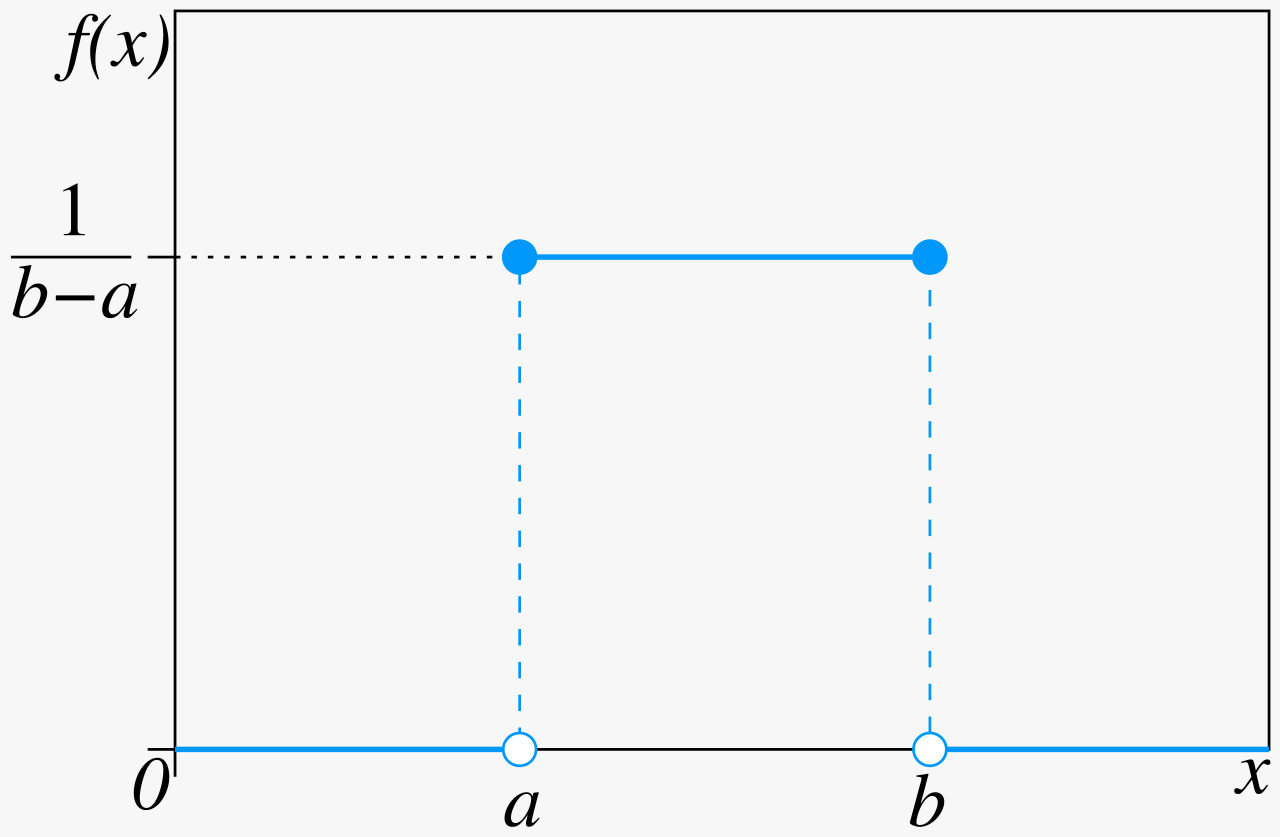
\includegraphics[width=0.5\textwidth]{distribuzione_continua_uniforme}
  	 		\end{figure}
  	 		\[
  	 		f(x) = \begin{cases}
  	 			\frac{1}{b-a} \quad x \in [a, b] \\
  	 			0 \quad x \notin [a, b]
  	 		\end{cases}
  	 		\]
  	 		e la funzione di ripartizione:
  	 		\[
  	 		F_X(t) = \int_{-\infty}^{t}f(x)dx = \int_{-\infty}^{t}\frac{1}{b-a}dx = \int_{a}^{t}\frac{1}{b-a}dx=\frac{t-a}{b-a}
  	 		\]
  	 		allora:
  	 		\[
  	 		F_X(t) = \begin{cases}
  	 			0 \quad t < a \\ \quad \\
  	 			\dfrac{t-a}{b-a} \quad a \leq t < b \\ \quad \\
  	 			1 \quad t \geq b
  	 		\end{cases}
  	 		\]
  	 		Poiche' $X$ assume valori in $[a,b]$ se $t < a$ l'evento $\{X\leq t\}$ e' impossibile, nel caso in cui $a \leq t \leq b$ e' l'integrale svolto precedentemente, se $t > b$ allora:
  	 		\[
  	 		F_X(t) = \int_{a}^{b}\frac{1}{b-a}dx = \frac{b-a}{b-a}= 1
  	 		\]
   	 	\end{example}
  	 	\subsection{Attesa e varianza di una variabile aleatoria continua}
  	 	\paragraph{Attesa di una v.a. continua} \quad \\
  	 	L'attesa di una variabile aleatoria continua e' data da:
  	 	\[
  	 	E[X] = \int_{-\infty}^{+\infty}xf(x)dx
  	 	\]
  	 	a patto che:
  	 	\[
  	 	\int_{-\infty}^{+\infty}|x|f(x)dx < \infty
  	 	\]
  	 	\paragraph{Varianza di una v.a. continua} \quad \\
  	 	La varianza di una variabile aleatoria continua e' data da:
  	 	\[
  	 	Var[X] = \int_{-\infty}^{+\infty}(x - \mu)^2f(x)dx
  	 	\]
  	 	ove $\mu = E[X]$ ed e' ancora vero che:
  	 	\[
  	 	Var[X] = E[X^2] - E[X]^2
  	 	\]
  	 	\begin{example}{\nmu Attesa e varianza della distribuzione uniforme}{}
  	 		Calcoliamo l'attesa:
  	 		\begin{align*}
  	 		E[X] &= \int_{a}^{b}\frac{x}{b-a}dx = \\ &= \frac{1}{b-a}\frac{1}{2}\big[x^2\big]^{x=b}_{x=a} =\\ &=\frac{1}{2}\frac{1}{b-a}(b^2-a^2) = \\ &= \frac{1}{b-a}\frac{1}{2}(b-a)(b+a) = \\ &= \frac{b+a}{2}
  	 		\end{align*}
  	 		Calcoliamo la varianza:
  	 		\begin{align*}
  	 		E[X^2] &= \int_{a}^{b}\frac{x^2}{b-a}dx = \\ &= \frac{1}{3}\frac{1}{b-a}\big[x^3\big]^{x=b}_{x=a} = \\  &= \frac{1}{b-a}\frac{1}{3}(b^3 - a^3) = \\ &= \frac{1}{3}(b^2 + ab + a^2)
  	 		\end{align*}
  	 		Quindi:
  	 		\begin{align*}
  	 		Var[X] &= \frac{1}{3}(b^2 + ab + a^2) - \frac{(a+b)^2}{4} = \\ &= \frac{4b^2 + 4ab + 4a^2 - 3(a^2 + b^2 + 2ab)}{12} = \\ &= \frac{b^2 + a^2 - 2ab}{12} = \\ &= \frac{(b-a)^2}{12}
  	 		\end{align*}
  	 	\end{example}
\end{document}
